\label{a1}

\begin{figure}[H]
\centering
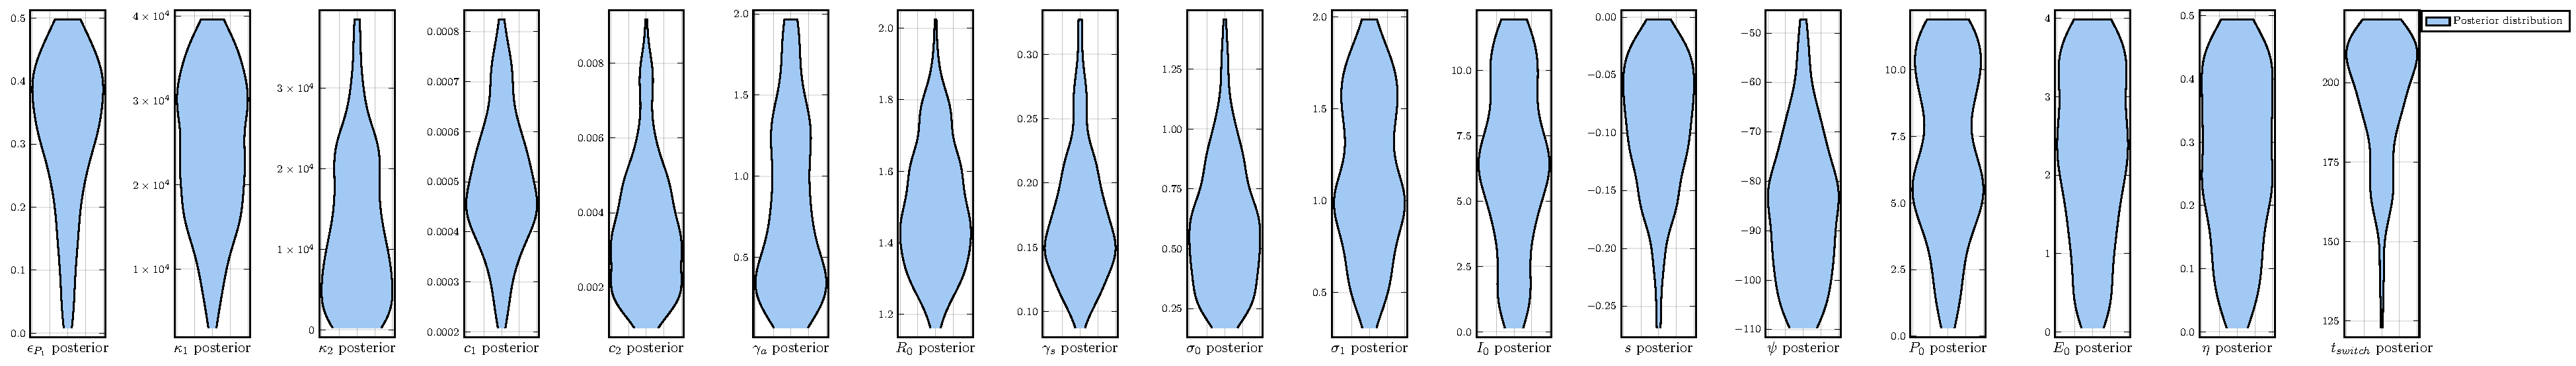
\includegraphics[width = 18 cm]{appendices/FigureS1.pdf}
\caption[Posterior distributions on inferred non-age structured model parameters for baseline model.]{\textbf{Posterior distributions on inferred non-age structured model parameters for baseline model}.Posteriors are composed of 200 candidate parameter sets from the particle filtering, the model was evaluated at these points for all future runs.}
\label{s1}
\end{figure}

\begin{figure}[H]
    \centering
    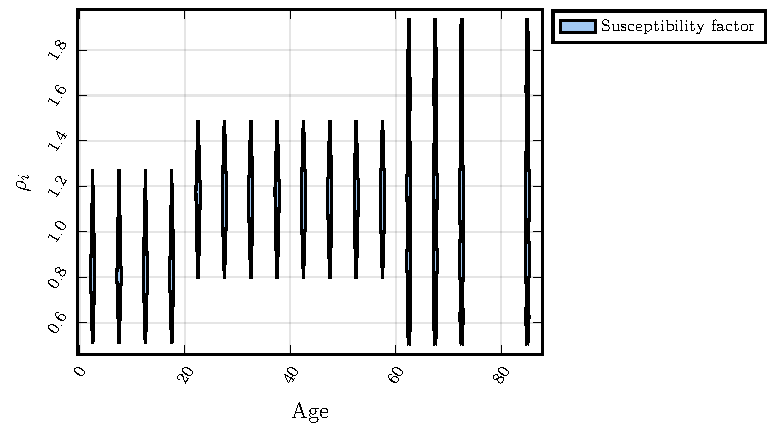
\includegraphics[width = 12 cm]{appendices/FigureS2.pdf}
    \caption{\textbf{Posterior distributions on inferred age-specific susceptibility modifier parameter $\rho_i$ for baseline model}. Three age-specific susceptibility parameters shown here, $\rho_1,\rho_2,\rho_3$, were also inferred from particle filtering on the case and mobility data, corresponding to the age brackets 0-20, 20-60, 60+.}
    \label{s2}
    \end{figure}
    
    \clearpage 
    
    \begin{figure}[H]
    \centering
    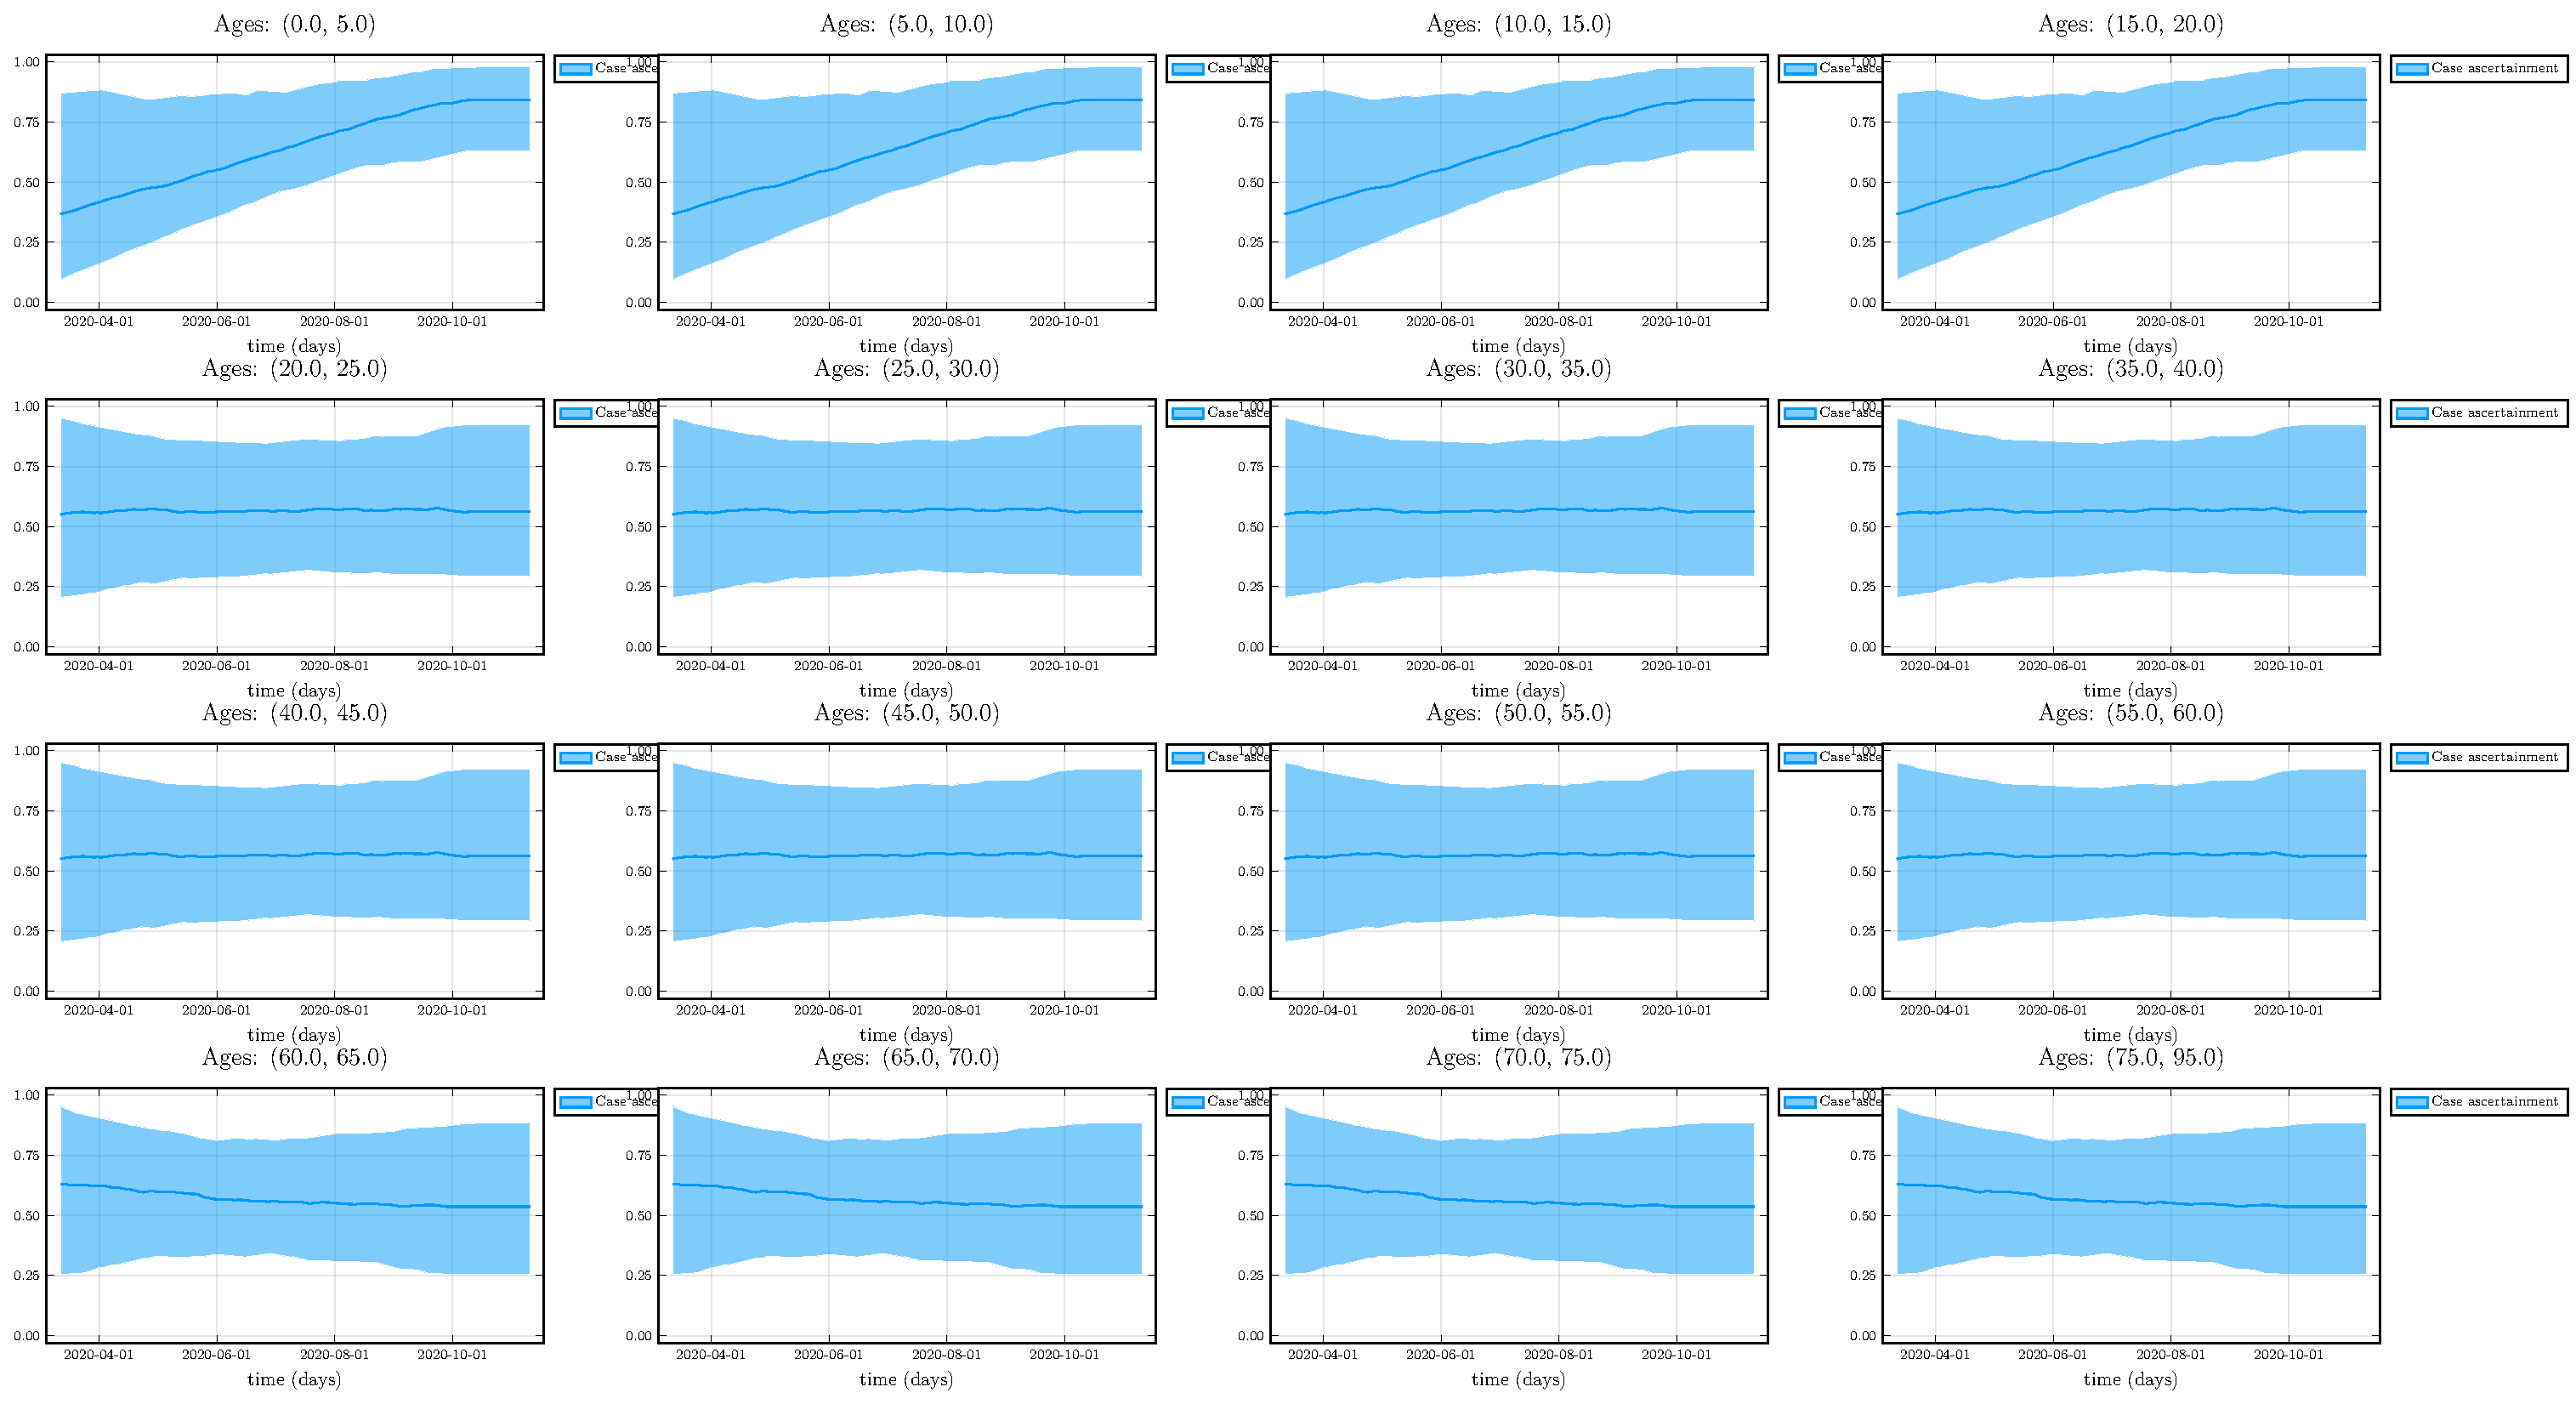
\includegraphics[width = 18 cm]{appendices/FigureS3.pdf}
    \caption[Posterior distributions on inferred age-specific ascertainment rate over time for baseline model.]{\textbf{Posterior distributions on inferred age-specific ascertainment rate over time for baseline model}. Time dependent ascertainment rates inferred from the data, corresponding to the fraction of actual cases detected by the Ontario testing system. }
    \label{s3}
    \end{figure}
    
    \clearpage 
    
    \begin{figure}[H]
    \centering
    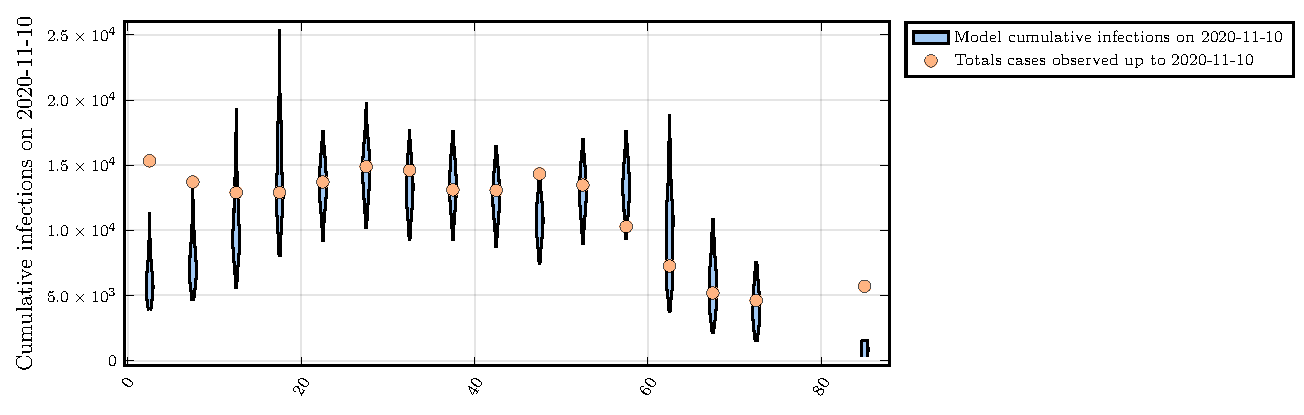
\includegraphics[width = 12 cm]{appendices/FigureS4.pdf}
    \caption[Empirical data of cumulative infections due to COVID-19 by age and model posterior predictions.]{\textbf{Empirical data of cumulative infections due to COVID-19 by age and model posterior predictions.} The age-specific total cases at the end of the fitting window, were used to calibrate the model, in an age dependent way. We used only three parameters to capture age specific effects and therefore trade-off some accuracy in the youngest and oldest age groups.}
    \label{s4}
    \end{figure}
    
    \clearpage 
    
    \begin{figure}[H]
    \centering
    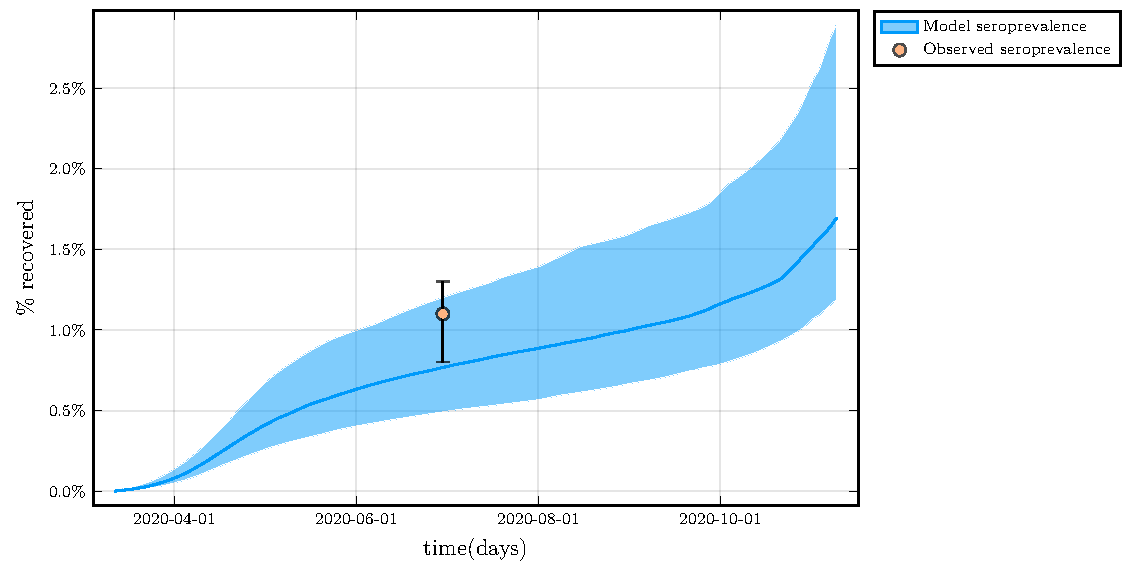
\includegraphics[width = 12 cm]{appendices/FigureS5.pdf}
    \caption[Average of model posterior population seropositivity over time, compared to empirical data.]{\textbf{Average of model posterior population seropositivity over time, compared to empirical data.} Total seroprevalence in Ontario was assessed during the month of June. We used this value to calibrate the model further.  }
    \label{s5}
    \end{figure}
    
    \clearpage 
    
    \begin{figure}[H]
    \centering
    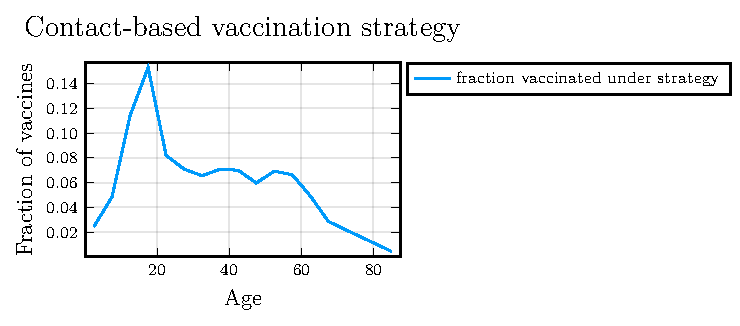
\includegraphics[width = 12 cm]{appendices/FigureS6.pdf}
    \caption[Age distribution of vaccination under the contact-based strategy.]{\textbf{Age distribution of vaccination under the contact-based strategy.} This strategy vaccinates proportionally to the leading eigenvector of the full contact matrix, $C(0)$, to vaccinate people who will, approximately, produce the most secondary infections in a linearized regime.}
    \label{s6}
    \end{figure}
    
    \clearpage 
    
    \begin{figure}[H]
    \centering
    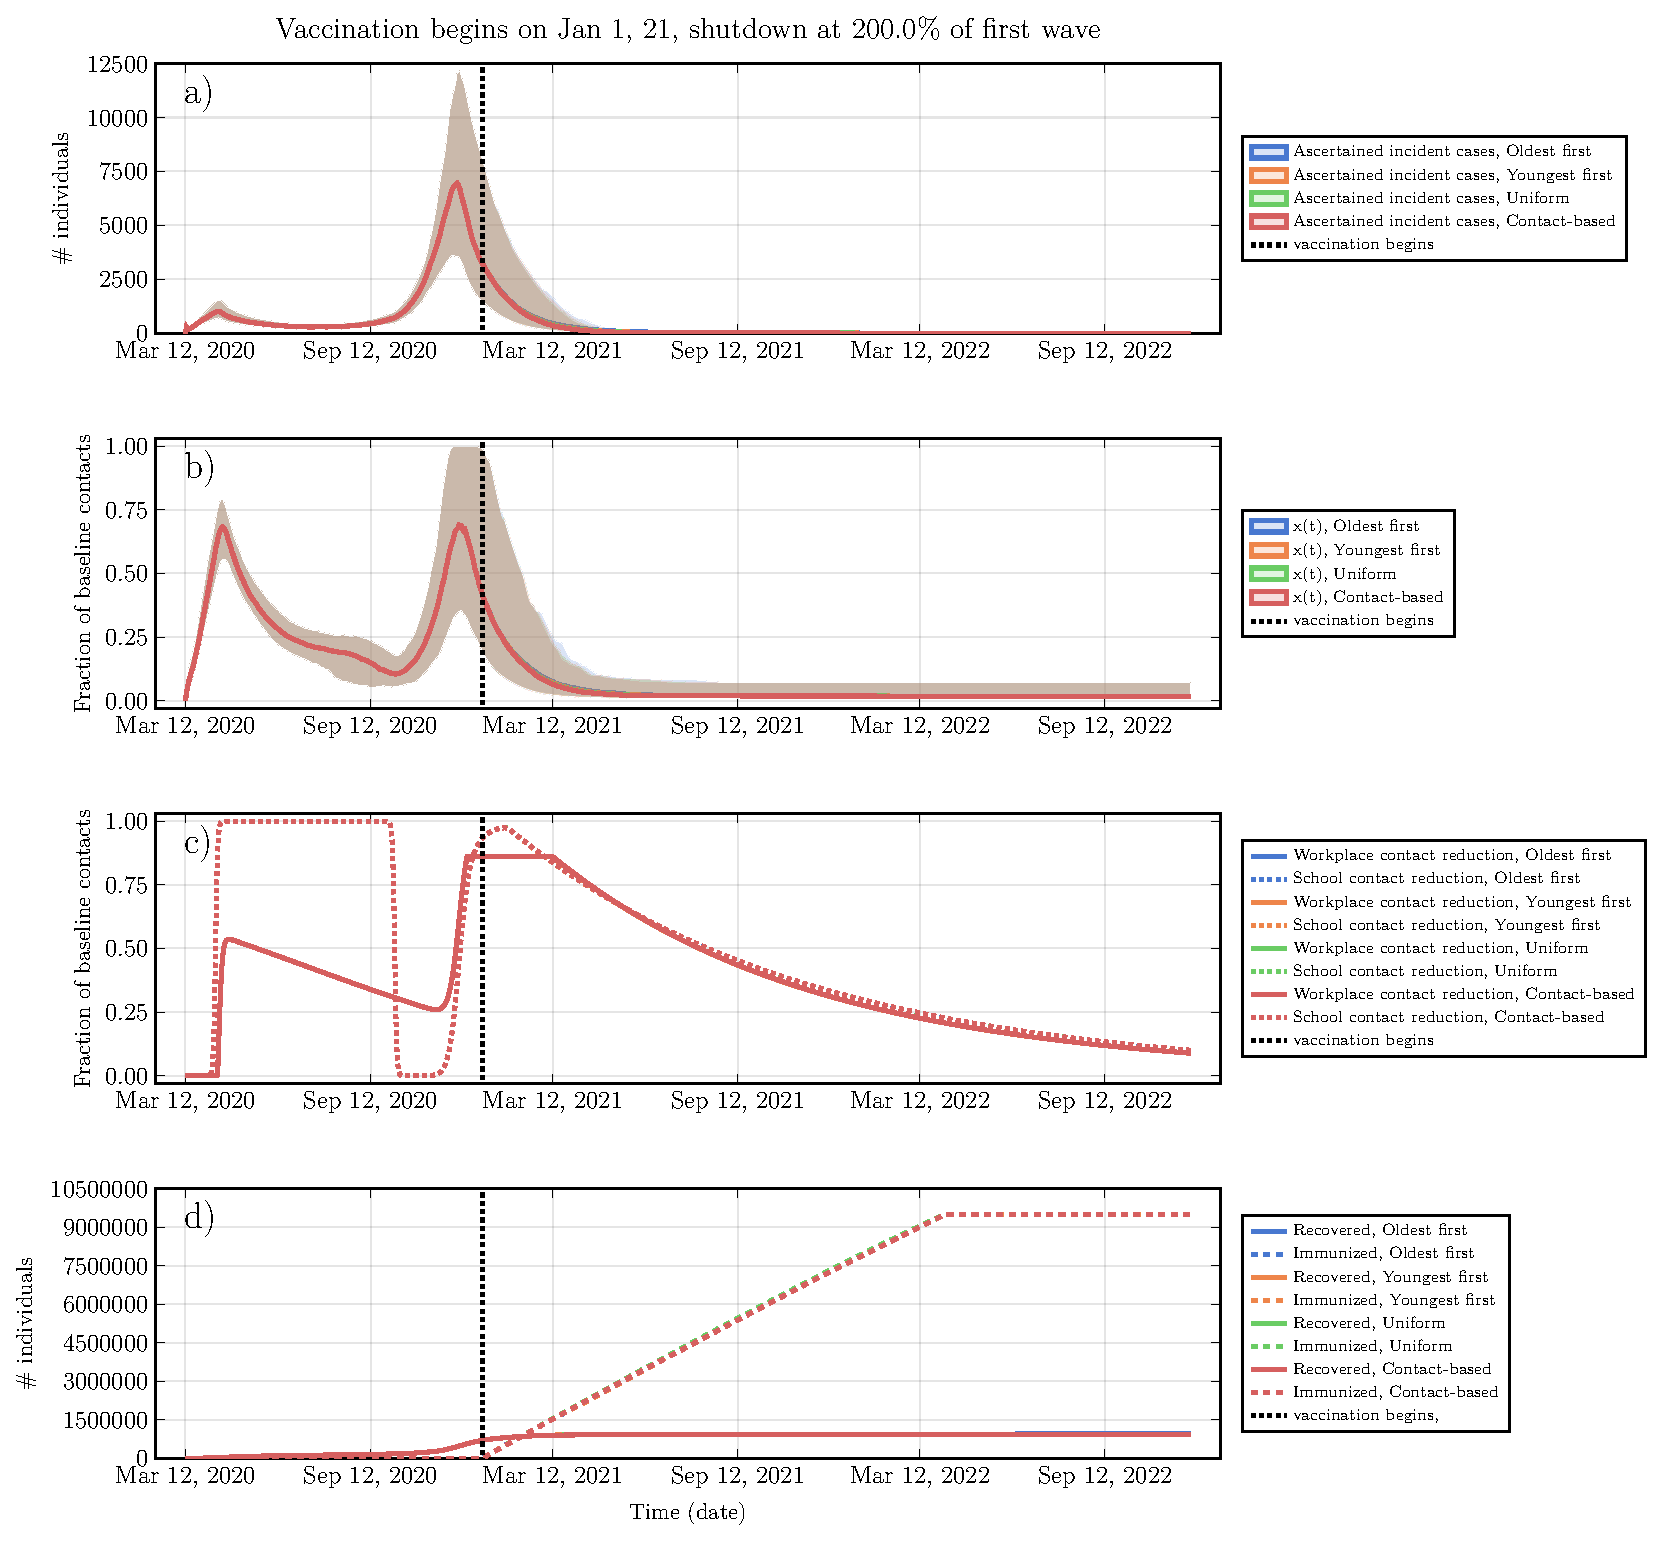
\includegraphics[width = 16 cm]{appendices/FigureS7.pdf}
    \caption[Social and epidemic dynamics for early vaccine availability and high vaccination rate.]{\textbf{Social and epidemic dynamics for early vaccine availability and high vaccination rate.} (a) Ascertained incident COVID-19 cases, (b) proportion $x$ of the population practicing NPIs, (c) Intensity of school and workplace closure, (d) percentage of population with natural or vaccine-derived immunity versus time. $T=200 \%$, $\psi_0=1.5 \%$ per week, vaccine available in January 2021.   Other parameters are in Table \ref{tab:params}.}
    \label{s7}
    \end{figure}
    
    \clearpage 
    
    \begin{figure}[H]
    \centering
    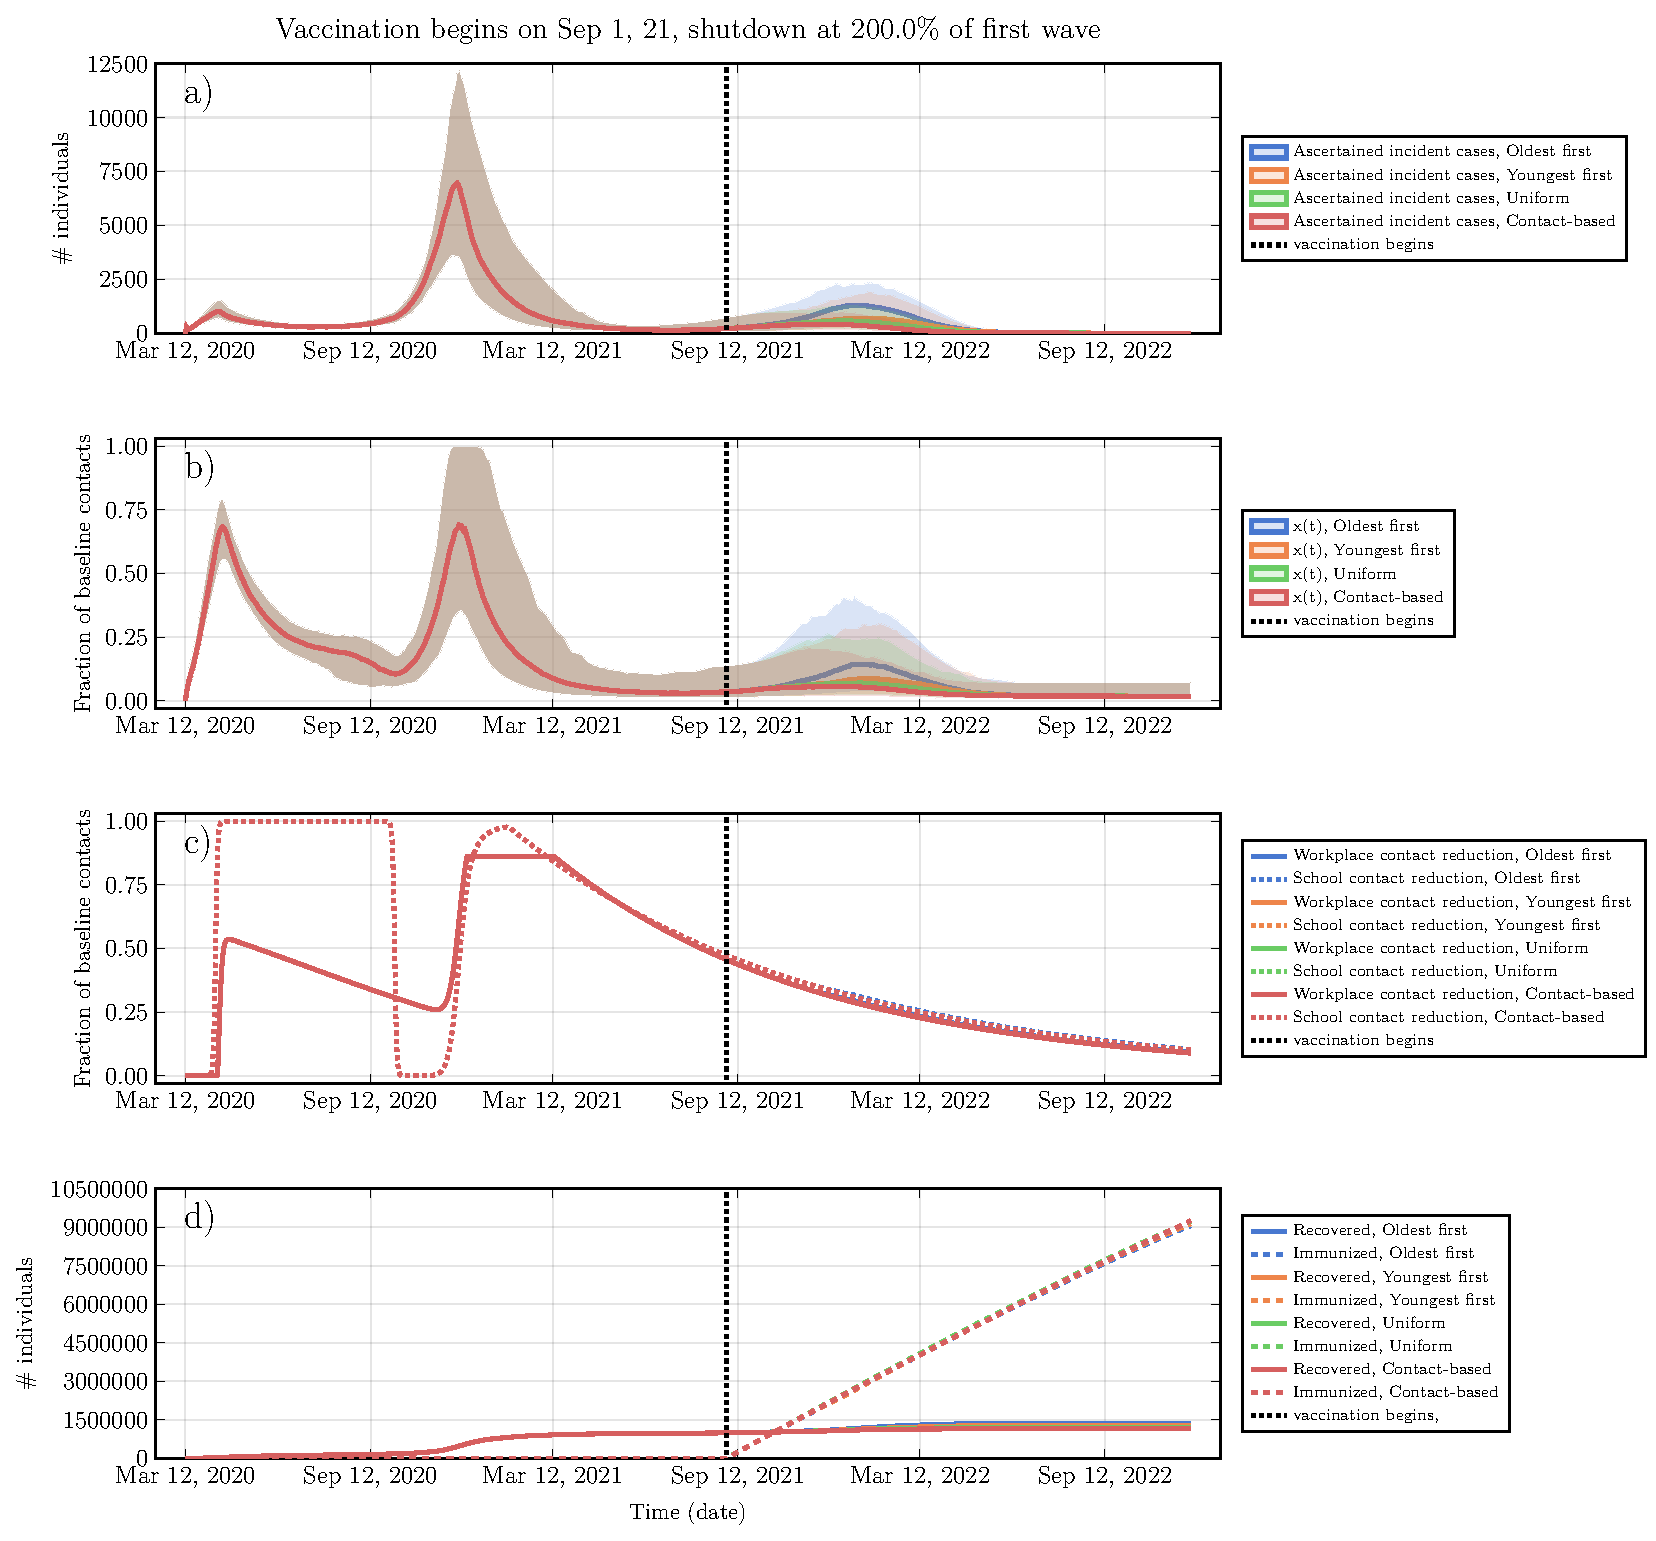
\includegraphics[width = 16 cm]{appendices/FigureS8.pdf}
    \caption[Social and epidemic dynamics for late vaccine availability and high vaccination rate.]{\textbf{Social and epidemic dynamics for late vaccine availability and high vaccination rate.} (a) Ascertained incident  COVID-19 cases, (b) proportion $x$ of the population practicing NPIs, (c) Intensity of school and workplace closure, (d) percentage of population with natural or vaccine-derived immunity versus time. $T=200 \%$, $\psi_0=1.5 \%$ per week, vaccine available in September 2021.   Other parameters are in Table \ref{tab:params}.}
    \label{s8}
    \end{figure}
    
    \clearpage 
    
    \begin{figure}[H]
    \centering
    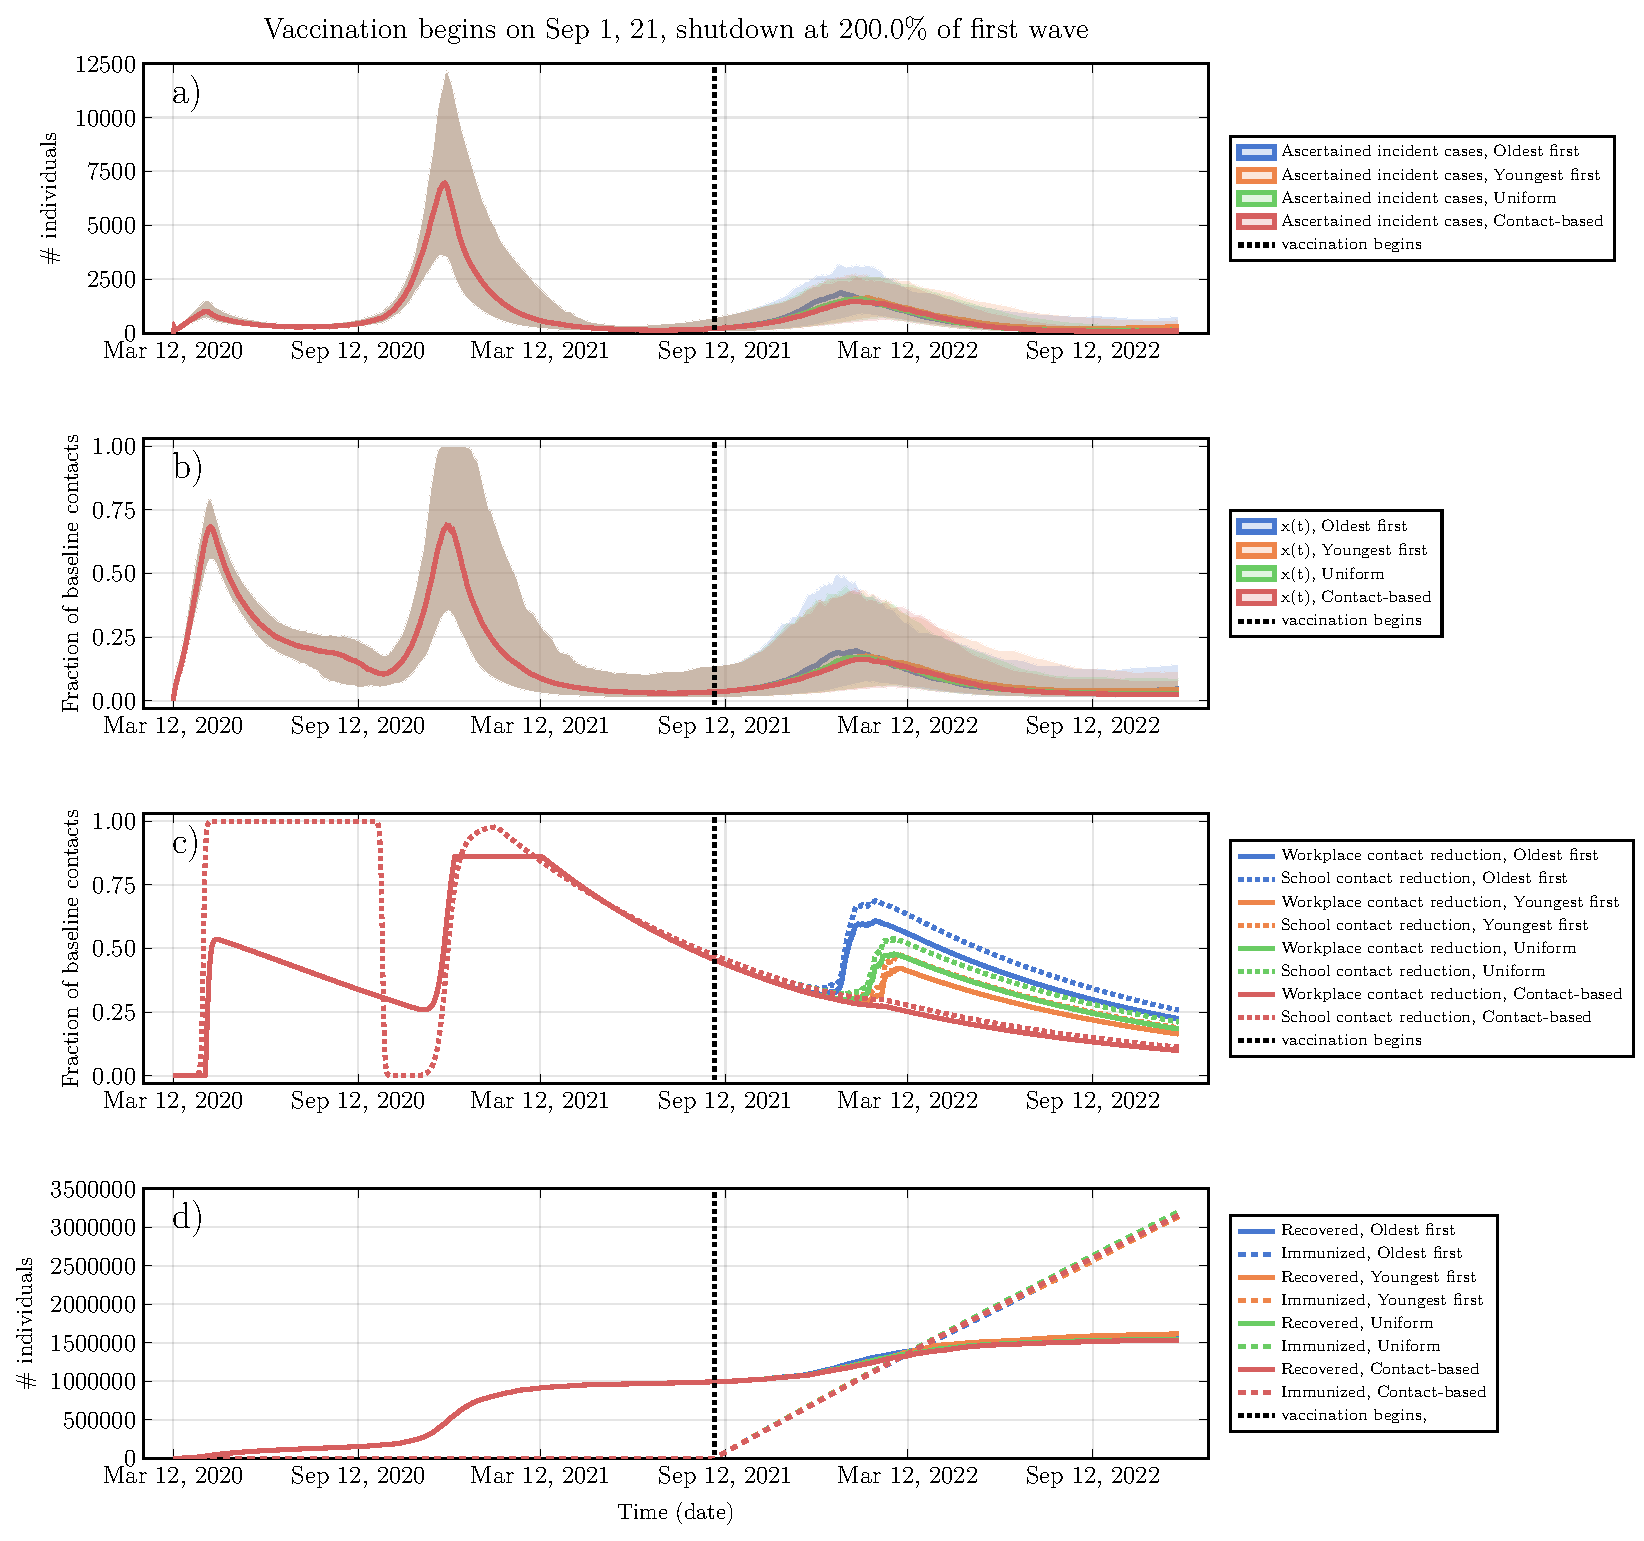
\includegraphics[width = 16 cm]{appendices/FigureS9.pdf}
    \caption[Social and epidemic dynamics for late vaccine availability and low vaccination rate.]{\textbf{Social and epidemic dynamics for late vaccine availability and low vaccination rate.} (a) Ascertained incident COVID-19 cases, (b) proportion $x$ of the population practicing NPIs, (c) Intensity of school and workplace closure, (d) percentage of population with natural or vaccine-derived immunity versus time. $T=200 \%$, $\psi_0=0.5 \%$ per week, vaccine available in September 2021.   Other parameters are in Table \ref{tab:params}.}
    \label{s9}
    \end{figure}
    
    
    \clearpage 
    
    \begin{figure}[H]
    \centering
    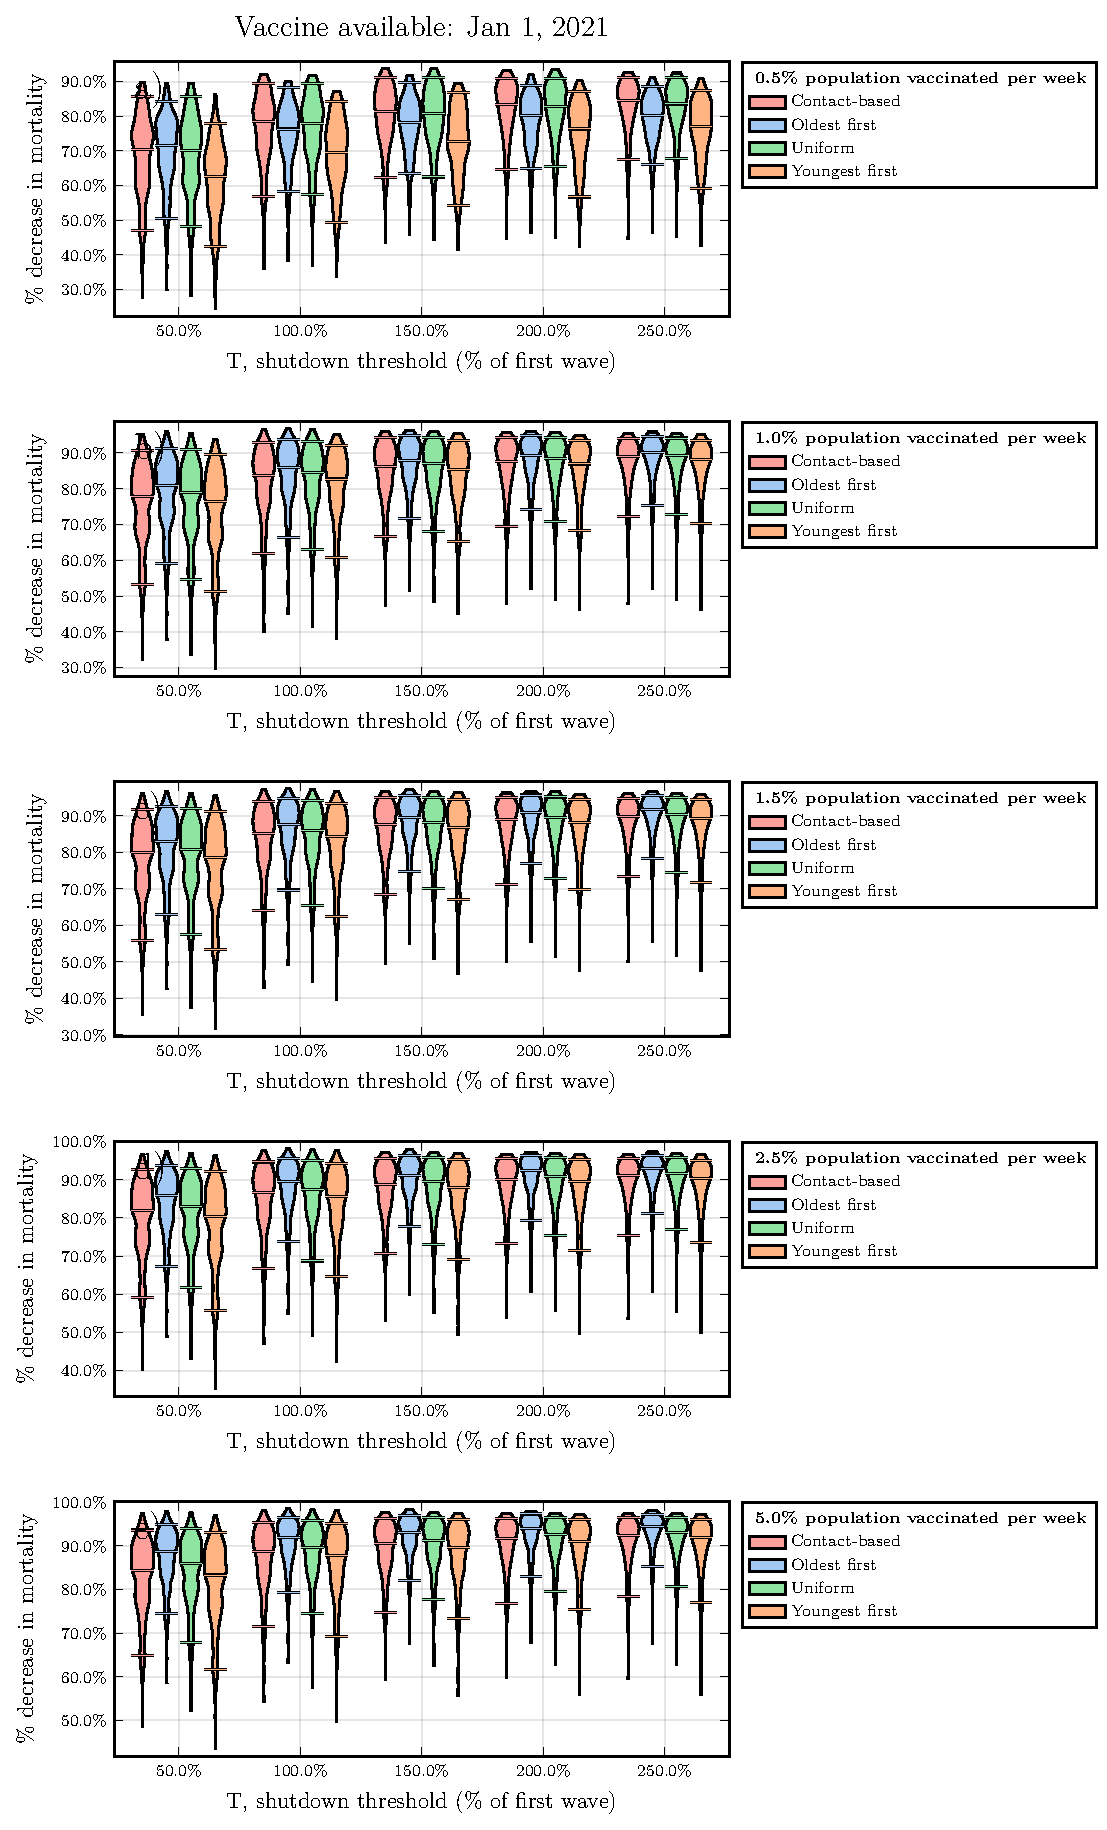
\includegraphics[width = 12 cm]{appendices/FigureS10.pdf}
    \caption[Mortality reductions under various values of $T$ and $\psi_0$, early vaccine availability.]{\textbf{Mortality reductions under various values of $T$ and $\psi_0$, early vaccine availability.} Violin plots of the percent reduction in mortality under the four vaccine strategies, relative to no vaccination, as a function of the vaccination rate $\psi_0$, for January 2021 availability. Horizontal lines represent median values of posterior model projections. Other parameter values in Table S1.  Percentage reductions are relative to no vaccination.  Projected number of deaths in the absence of vaccination were 35597.2 (CI: 57465.9,19507.9); 48518.8 (CI: 86853.9,28335.7), 61339.1 (CI: 106623.0,34613.5), 
    72007.3 (CI: 121754.0,40483.4); 80707.6 (CI: 126732.0,47755.4) after January 1, 2021, for T=50\%, 100\%, 150\%, 200\%, and 250\%, respectively. }
    \label{s10}
    \end{figure}
    
    
    
    
    \clearpage 
    
    
    \begin{figure}[H]
    \centering
    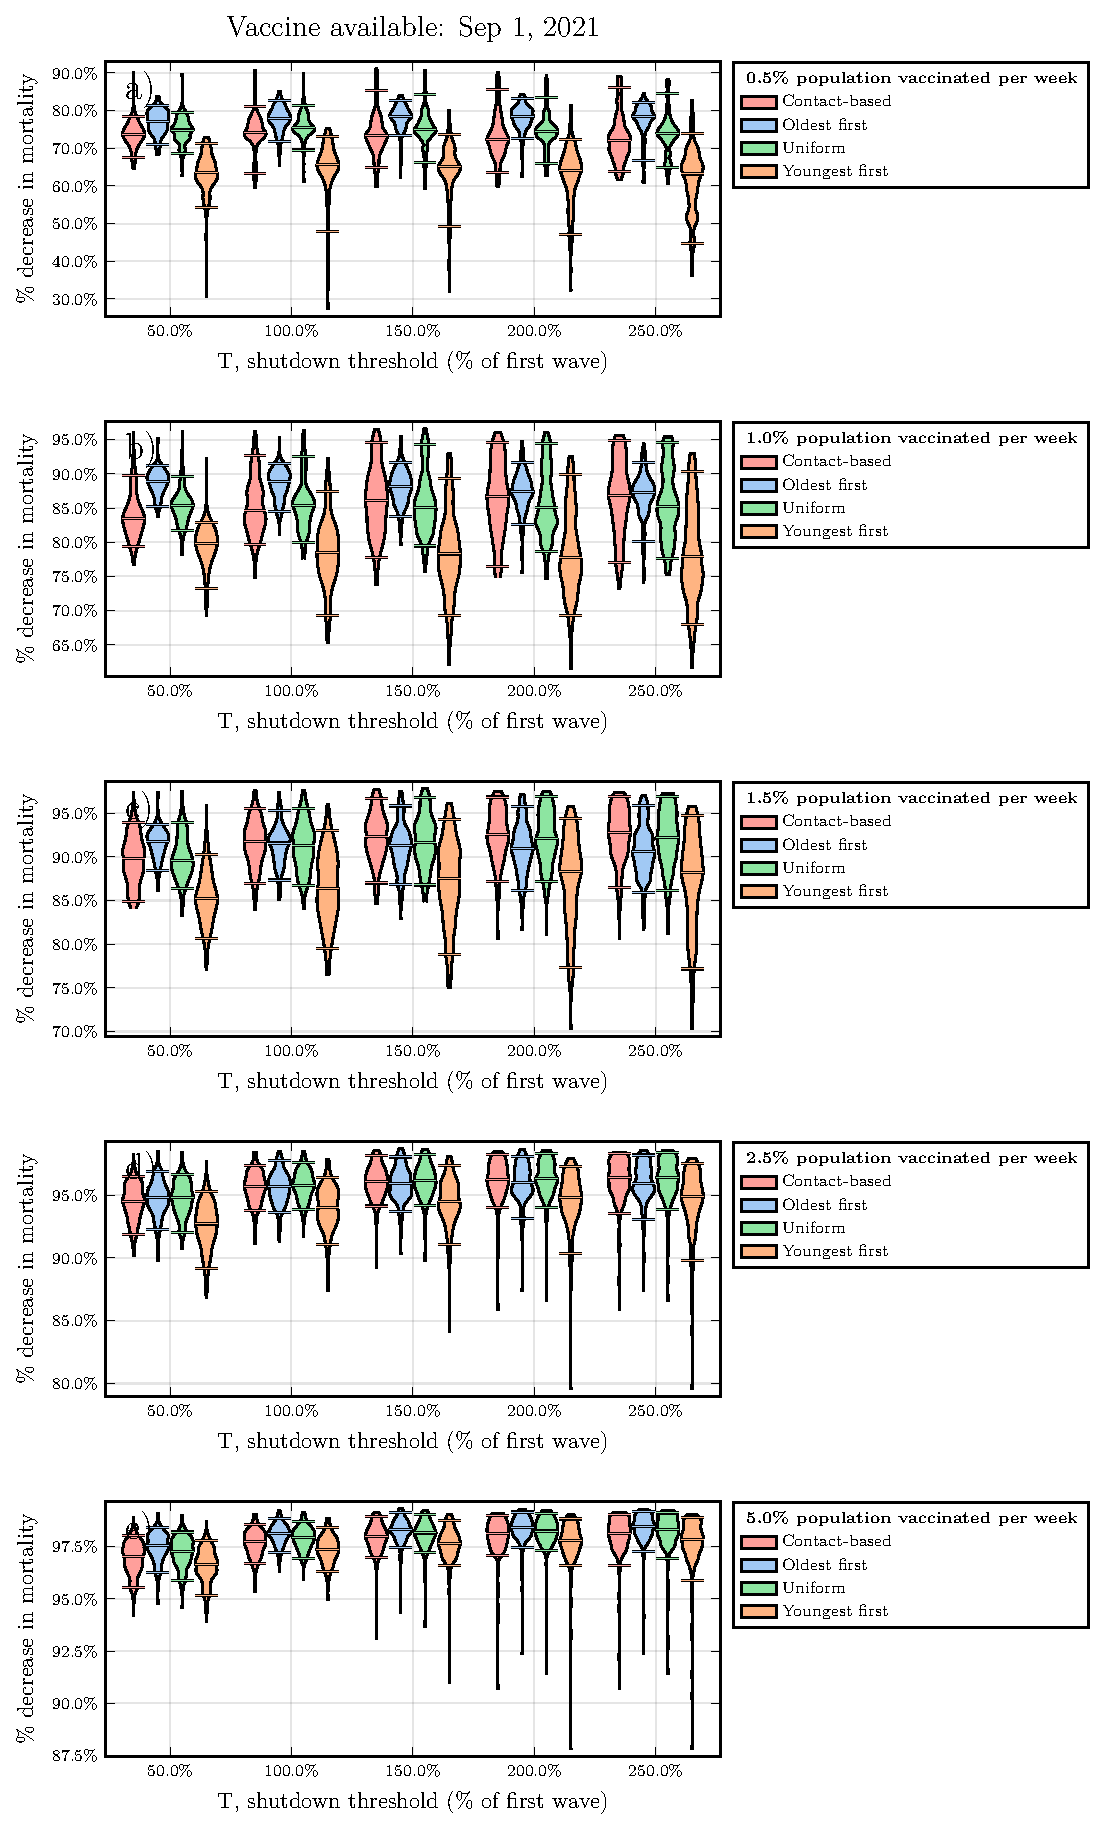
\includegraphics[width = 12 cm]{appendices/FigureS11.pdf}
    \caption[Mortality reductions under various values of $T$ and $\psi_0$, late vaccine availability.]{\textbf{Mortality reductions under various values of $T$ and $\psi_0$, late vaccine availability.} Violin plots of the percent reduction in mortality under the four vaccine strategies, relative to no vaccination, as a function of the vaccination rate $\psi_0$, for September 2021 availability. Horizontal lines represent median values of posterior model projections. Other parameter values in Table S1.  Percentage reductions are relative to no vaccination. Projected number of deaths in the absence of vaccination were 25478.8 (CI: 45679.0,13006.7); 39149.6 (CI: 73917.1,20290.9); 50775.1 (CI: 95451.2,25980.9); 60250.7 (CI: 108361.0,30721.9); 68594.0 (CI: 107157.0,36063.6) after September 1, 2021 for T=50\%, 100\%, 150\%, 200\%, and 250\%, respectively. }
    \label{s11}
    \end{figure}
    
    
    
    \clearpage 
    
    
    \begin{figure}[H]
    \centering
    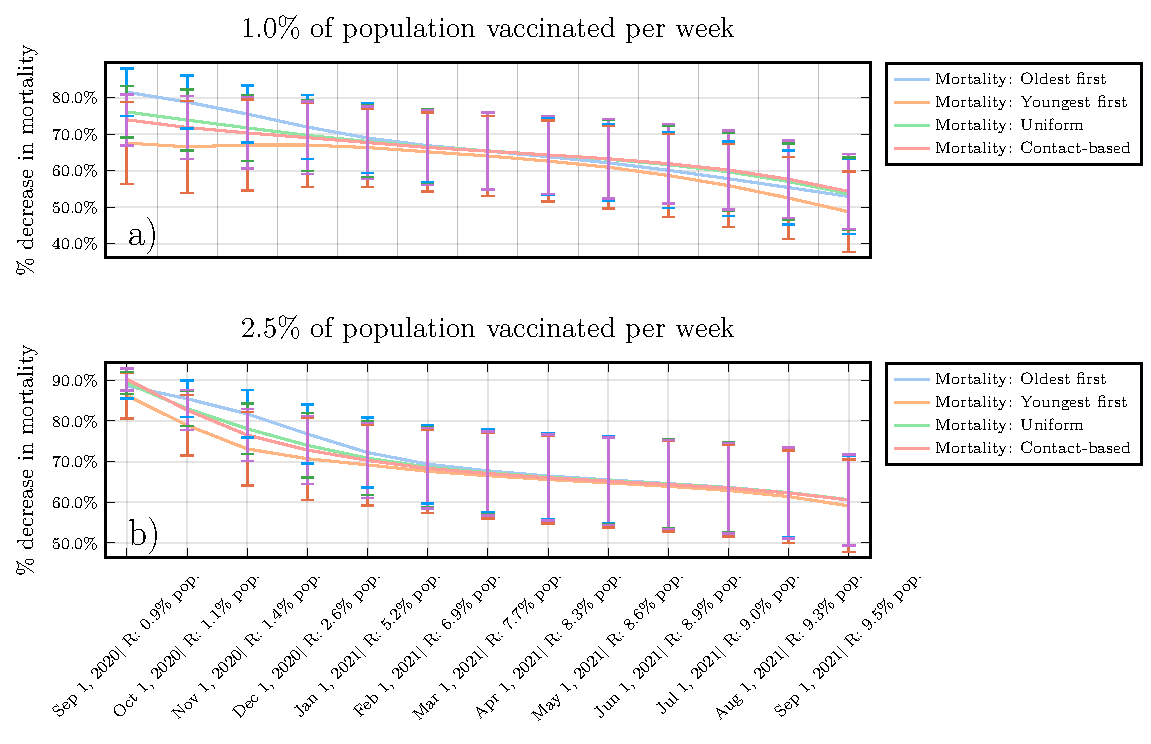
\includegraphics[width = 15 cm]{appendices/FigureS12.pdf}
    \caption[A higher level of natural immunity increases the relative advantage of transmission-interrupting strategies.]{\textbf{A higher level of natural immunity increases the relative advantage of transmission-interrupting strategies.}  Median and standard deviation of the percent reduction in mortality under the four vaccine strategies, relative to no vaccination, as a function of the vaccination start date and percent recovered at that time, for (a) $\phi_0=1.0 \%$ vaccinated per week and (b) $\phi_0=2.5 \%$ vaccinated per week.  Shutdown threshold $T=200 \%$,  and other parameter values in Appendix, Table S1.}
    \label{s12}
    \end{figure}
    
    \clearpage 
    
    \begin{figure}[H]
    \centering
    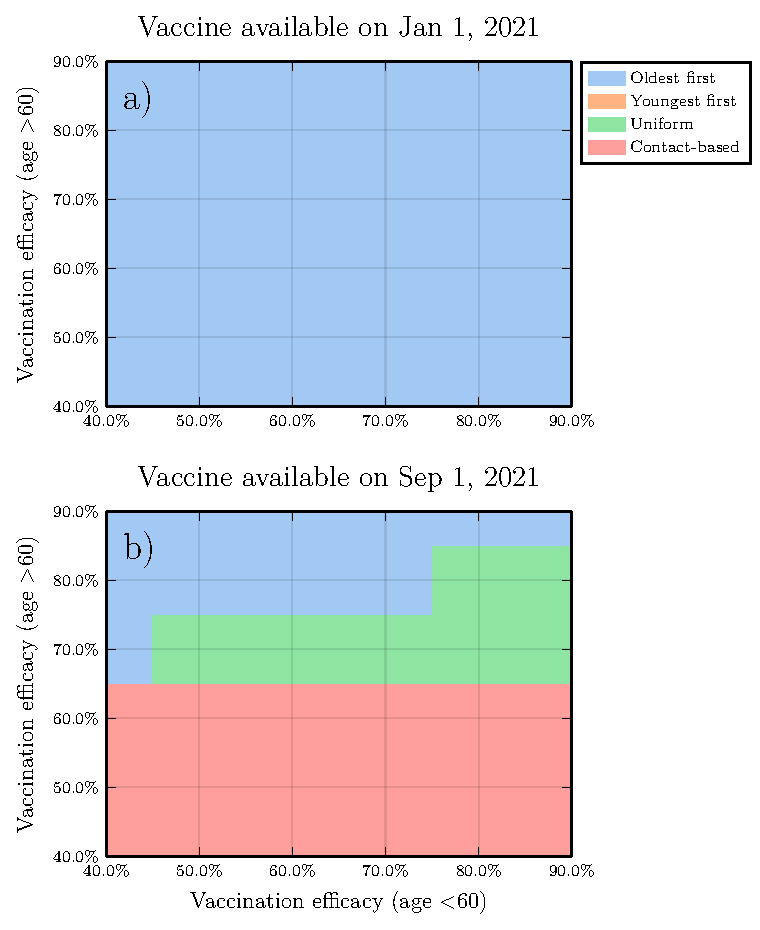
\includegraphics[width = 14 cm]{appendices/FigureS13.pdf}
    \caption[Sensitivity analysis exploring a range of vaccine efficacy values, for vaccination rate $\phi_0=2.5 \%$ per week.]{\textbf{Sensitivity analysis exploring a range of vaccine efficacy values, for vaccination rate $\phi_0=2.5 \%$ per week.} Subpanels are parameter planes for January and September availability showing the vaccination strategy that reduces COVID-19 mortality the most as a function of vaccine efficacy in $60+$ year-olds versus vaccine efficacy in other age groups. Other parameter values as in Table S1.}
    \label{s13}
    \end{figure}
    
    \clearpage 
    
    \begin{figure}[H]
    \centering
    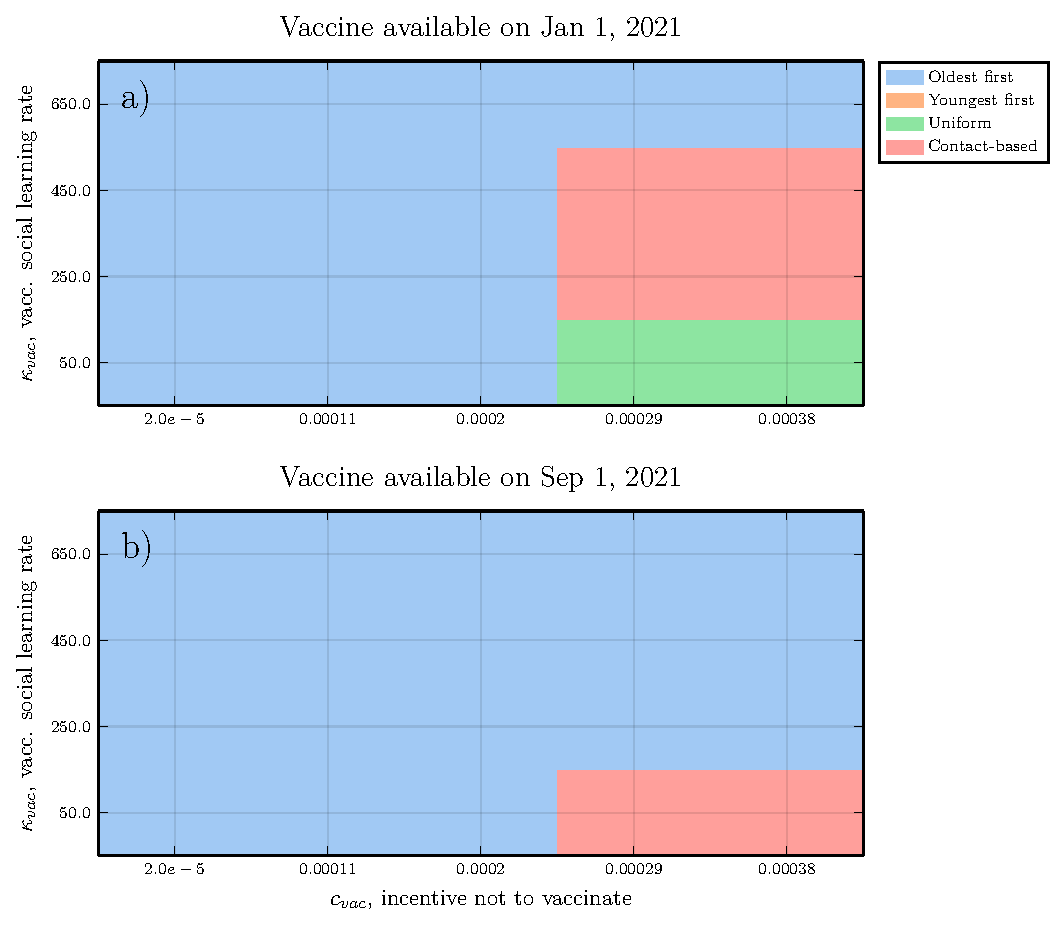
\includegraphics[width = 14 cm]{appendices/FigureS14.pdf}
    \caption[Sensitivity analysis exploring impact of vaccinating behaviour dynamics.]{\textbf{Sensitivity analysis exploring impact of vaccinating behaviour dynamics.} $\phi_0 = 2.5 \%$ per week, $T=200 \%$. Subpanels are parameter planes for January and September availability showing the vaccination strategy that reduces COVID-19 mortality the most as a function of vaccine social learning rate $\kappa_{vac}$ and vaccine cost parameter $c_{vac}$. Other parameter values as in Table S1.}
    \label{s14}
    \end{figure}
    
    \clearpage 
    
    \begin{figure}[H]
    \centering
    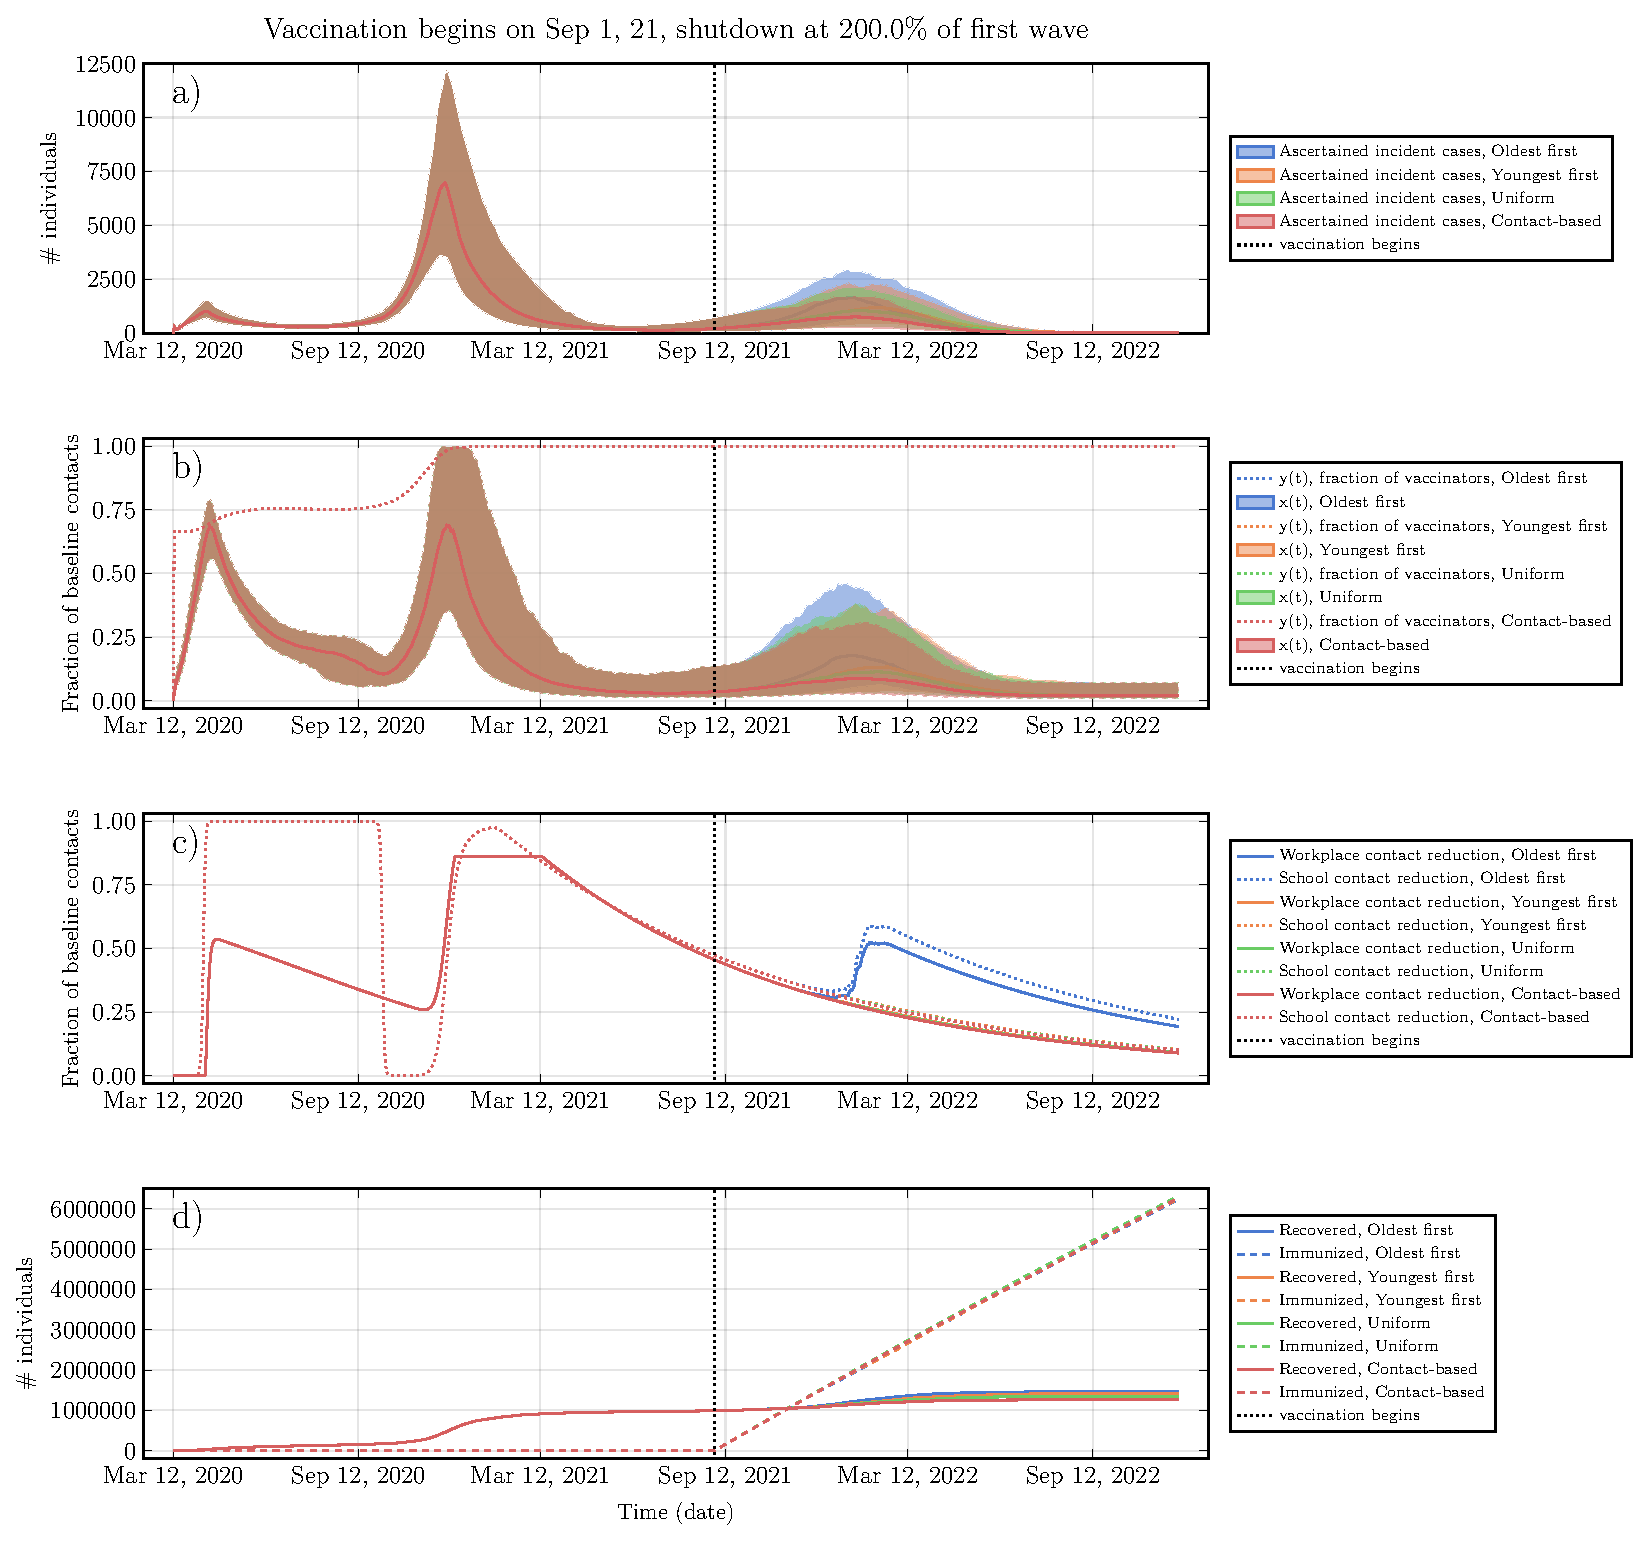
\includegraphics[width = 16 cm]{appendices/FigureS15.pdf}
    \caption[Epidemic dynamics and social dynamics for both NPI adherence and vaccinating behaviour, when vaccine cost is small, $c_{vac}=1.1\times 10^{-4}$.]{\textbf{Epidemic dynamics and social dynamics for both NPI adherence and vaccinating behaviour, when vaccine cost is small, $c_{vac}=1.1\times 10^{-4}$.} (a) Ascertained incident COVID-19 cases, (b) proportion $x$ of the population practicing NPIs, (c) Intensity of school and workplace closure, (d) percentage of population with natural or vaccine-derived immunity versus time. $T=200 \%$, $\psi_0=1.0 \%$ per week (maximum rate in absence of vaccine refusal), vaccine available in September 2021, $\kappa_{vac}=50$/day.   Other parameters are in Table \ref{tab:params}.}
    \label{s15}
    \end{figure}
    
    \clearpage 
    
    \begin{figure}[H]
    \centering
    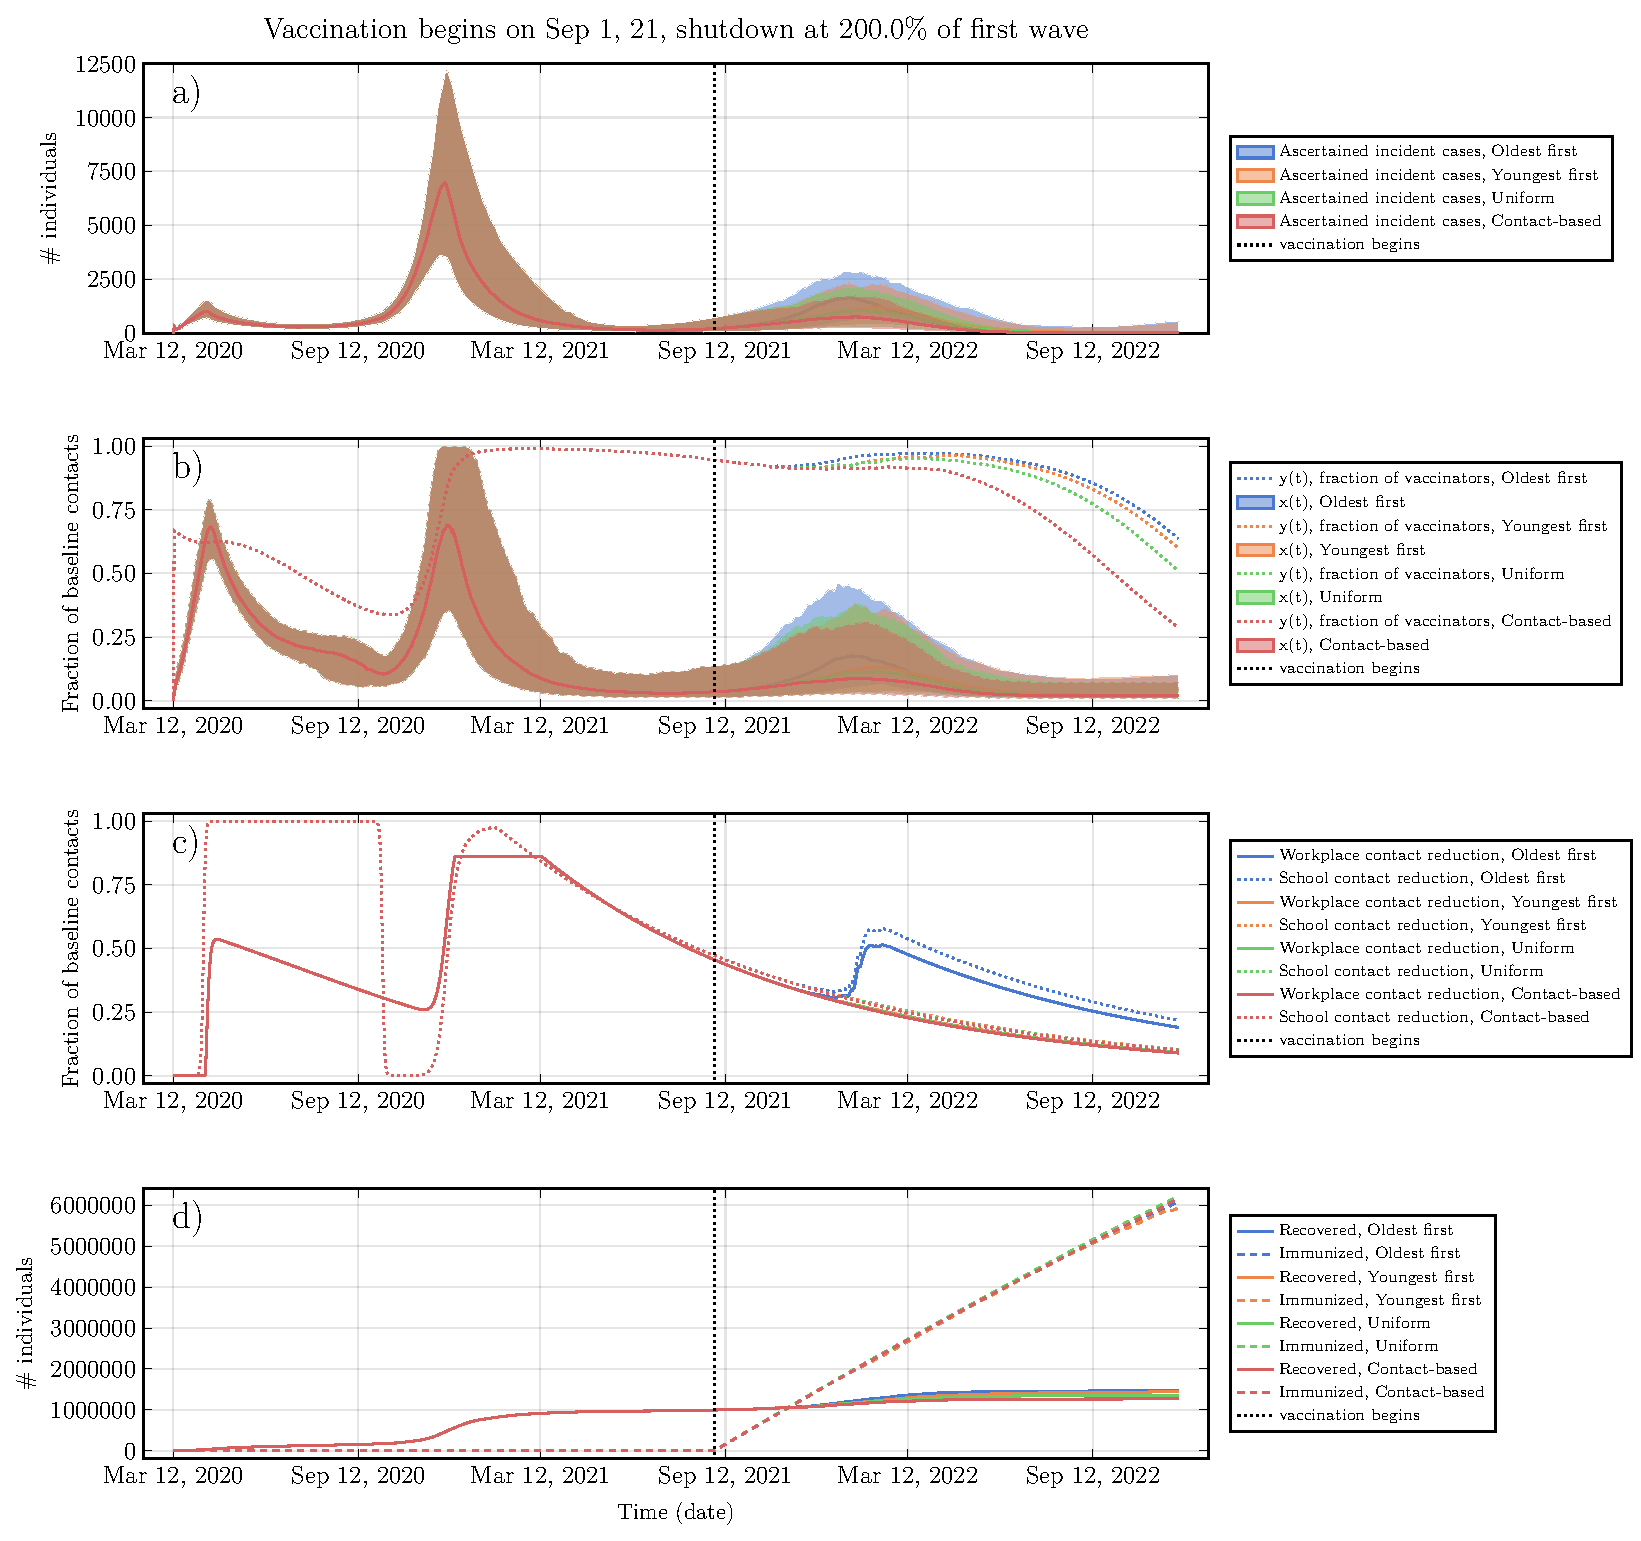
\includegraphics[width = 16 cm]{appendices/FigureS16.pdf}
    \caption[Epidemic dynamics and social dynamics for both NPI adherence and vaccinating behaviour, when vaccine cost is moderate, $c_{vac}=2.9\times 10^{-4}$.]{\textbf{Epidemic dynamics and social dynamics for both NPI adherence and vaccinating behaviour, when vaccine cost is moderate, $c_{vac}=2.9\times 10^{-4}$.} (a) Ascertained incident COVID-19 cases, (b) proportion $x$ of the population practicing NPIs, (c) Intensity of school and workplace closure, (d) percentage of population with natural or vaccine-derived immunity versus time. $T=200 \%$, $\psi_0=1.0 \%$ per week (maximum rate in absence of vaccine refusal), vaccine available in September 2021, $\kappa_{vac}=50$/day.   Other parameters are in Table \ref{tab:params}.}
    \label{s16}
    \end{figure}
    
    \clearpage 
    
    \begin{figure}[H]
    \centering
    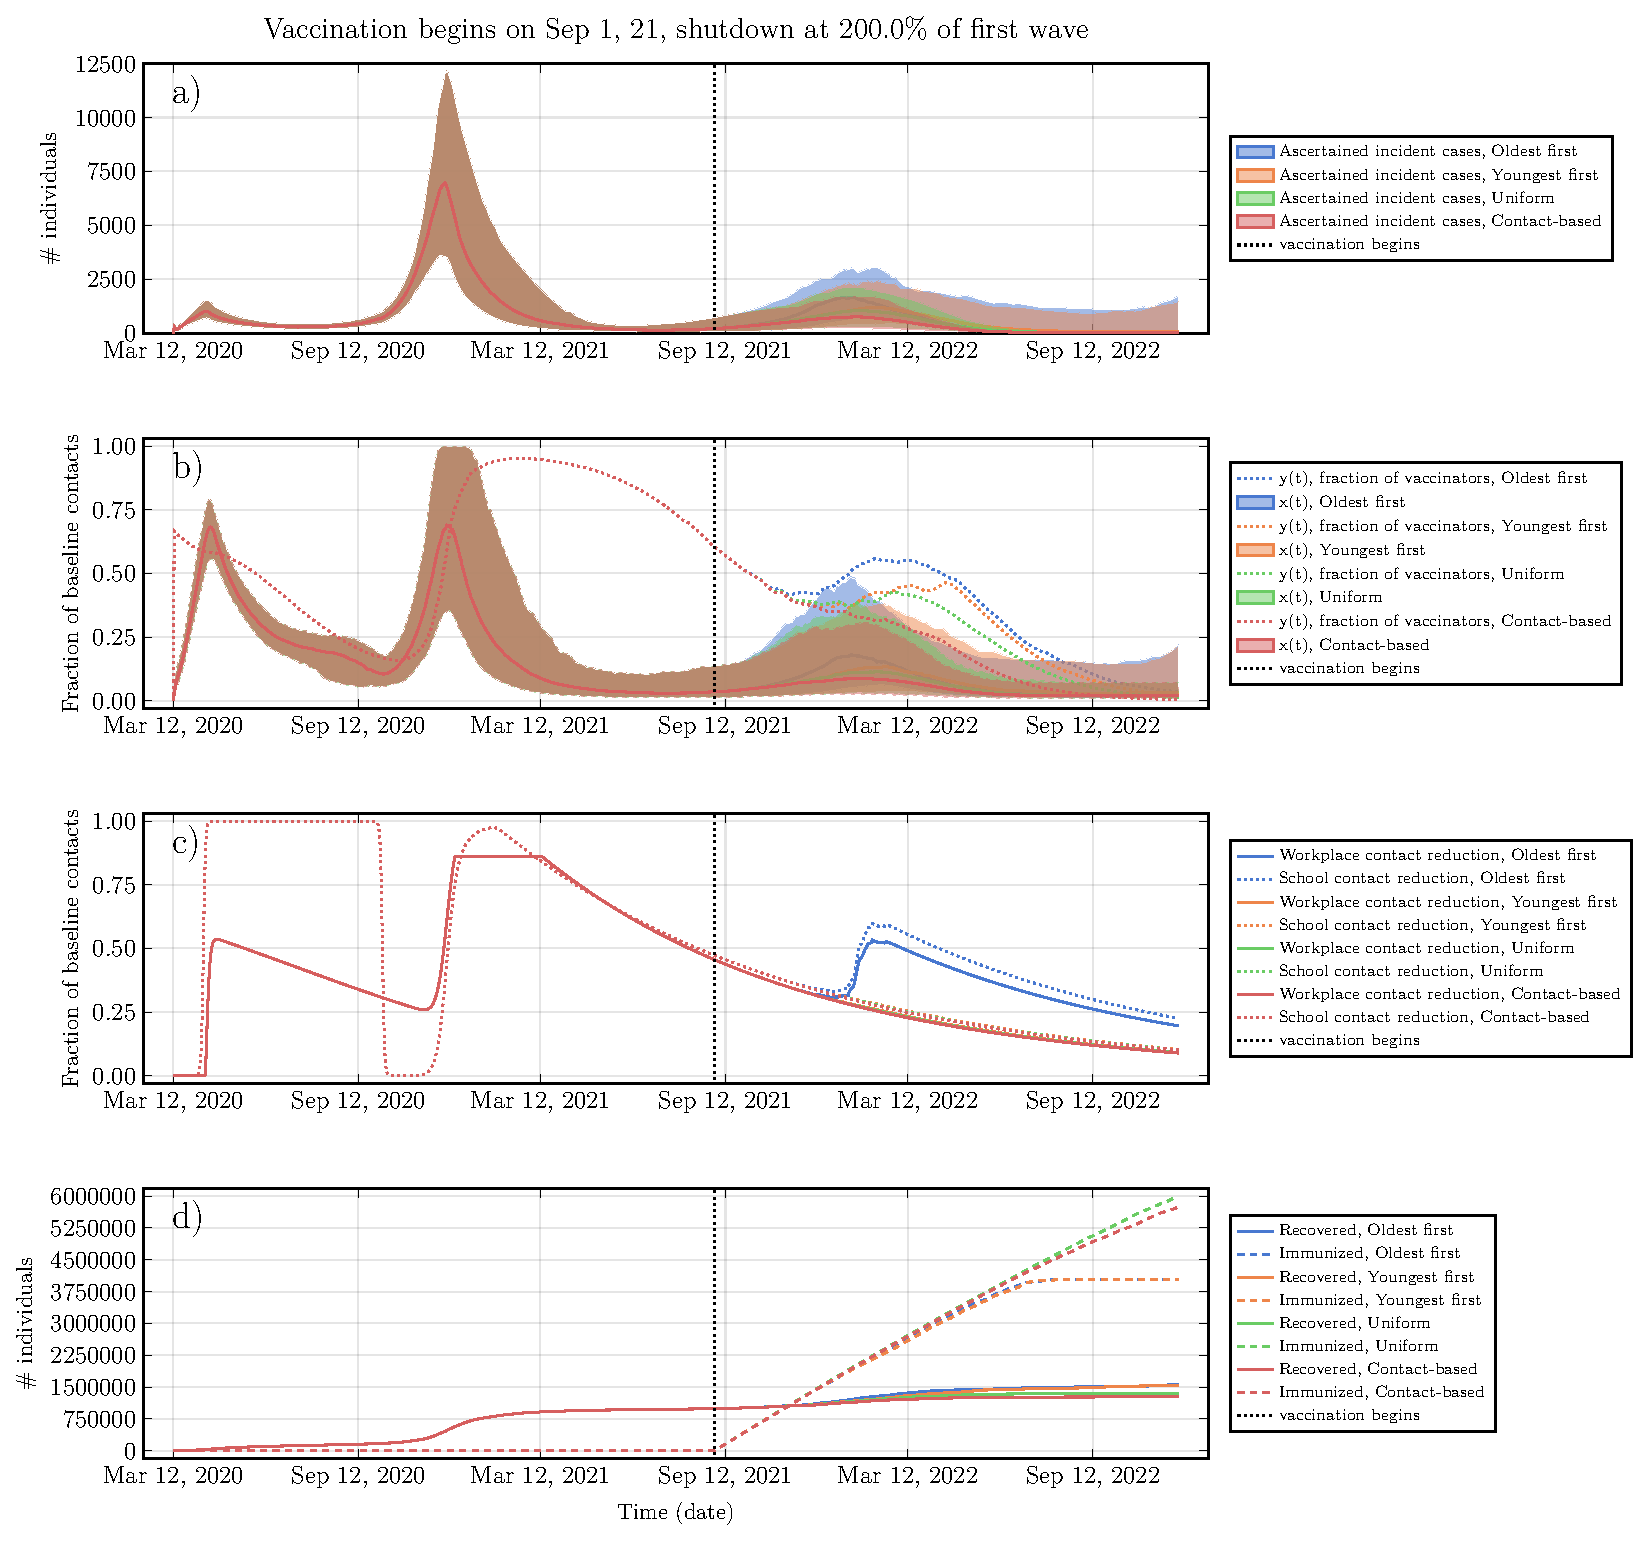
\includegraphics[width = 16 cm]{appendices/FigureS17.pdf}
    \caption[Epidemic dynamics and social dynamics for both NPI adherence and vaccinating behaviour, when vaccine cost is high, $c_{vac}=3.8\times 10^{-4}$.]{\textbf{Epidemic dynamics and social dynamics for both NPI adherence and vaccinating behaviour, when vaccine cost is high, $c_{vac}=3.8\times 10^{-4}$.} (a) Ascertained incident COVID-19 cases, (b) proportion $x$ of the population practicing NPIs, (c) Intensity of school and workplace closure, (d) percentage of population with natural or vaccine-derived immunity versus time. $T=200 \%$, $\psi_0=1.0 \%$ per week (maximum rate in absence of vaccine refusal), vaccine available in September 2021, $\kappa_{vac}=50$/day. Other parameters are in Table \ref{tab:params}.}
    \label{s17}
    \end{figure}
    
    \clearpage 
    
    \begin{figure}[H]
    \centering
    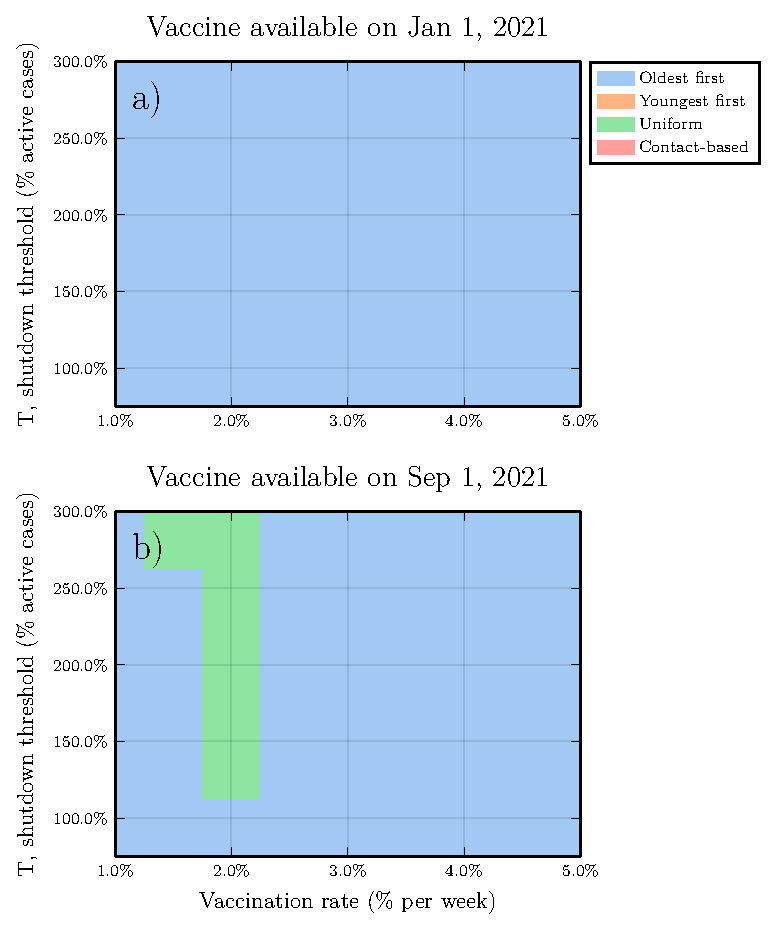
\includegraphics[width = 14 cm]{appendices/FigureS18.pdf}
    \caption[Sensitivity analysis for the scenario where $R_0=2.5$ for December 2020 onward.]{\textbf{Sensitivity analysis for the scenario where $R_0=2.5$ for December 2020 onward.} Subpanels are (left) parameter planes for January and September availability showing the vaccination strategy that prevents the most COVID-19 deaths as a function of $T$ and $\psi_0$, and (right) percentage reductions in mortality. Other parameter values are as in Table S1.}
    \label{s18}
    \end{figure}
    
    \clearpage 
    
    \begin{figure}[H]
    \centering
    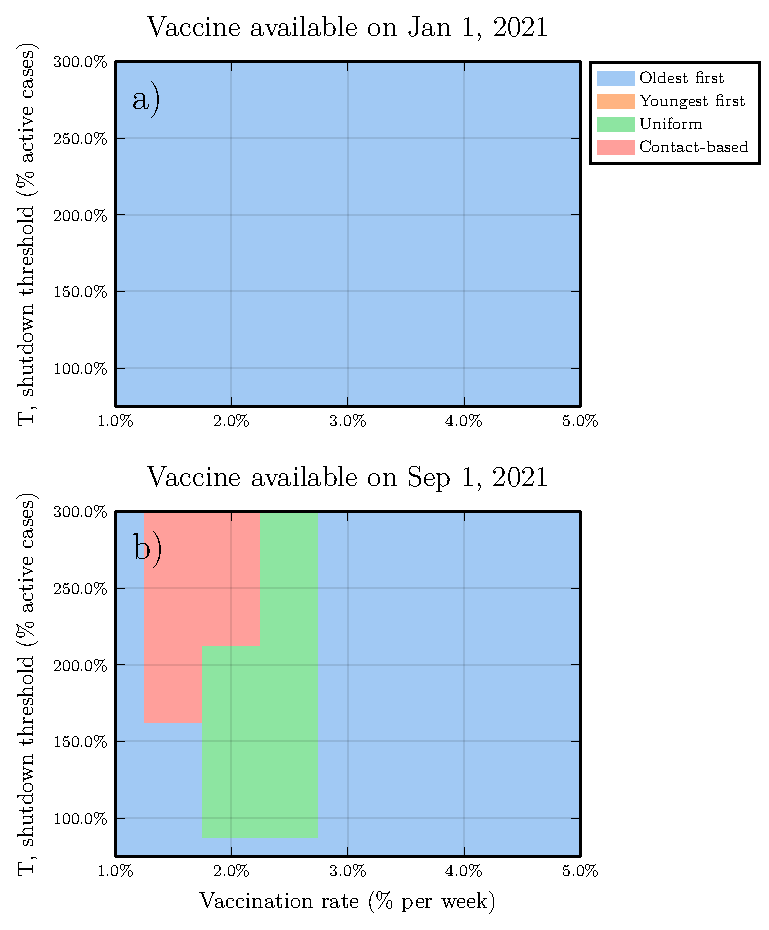
\includegraphics[width = 14 cm]{appendices/FigureS19.pdf}
    \caption[Sensitivity analysis for the scenario of $30 \%$ heightened ascertainment across all ages from December 2020 onward.]{\textbf{Sensitivity analysis for the scenario of $30 \%$ heightened ascertainment across all ages from December 2020 onward.} Subpanels are parameter planes for January and September availability showing the vaccination strategy that reduces COVID-19 mortality the most as a function of $T$ and $\psi_0$ (left) and the corresponding posterior parameter distributions for the refitted parameters (right).  Other parameter values as in Table S1.}
    \label{s19}
    \end{figure}
    
    \clearpage 
    
    \begin{figure}[H]
    \centering
    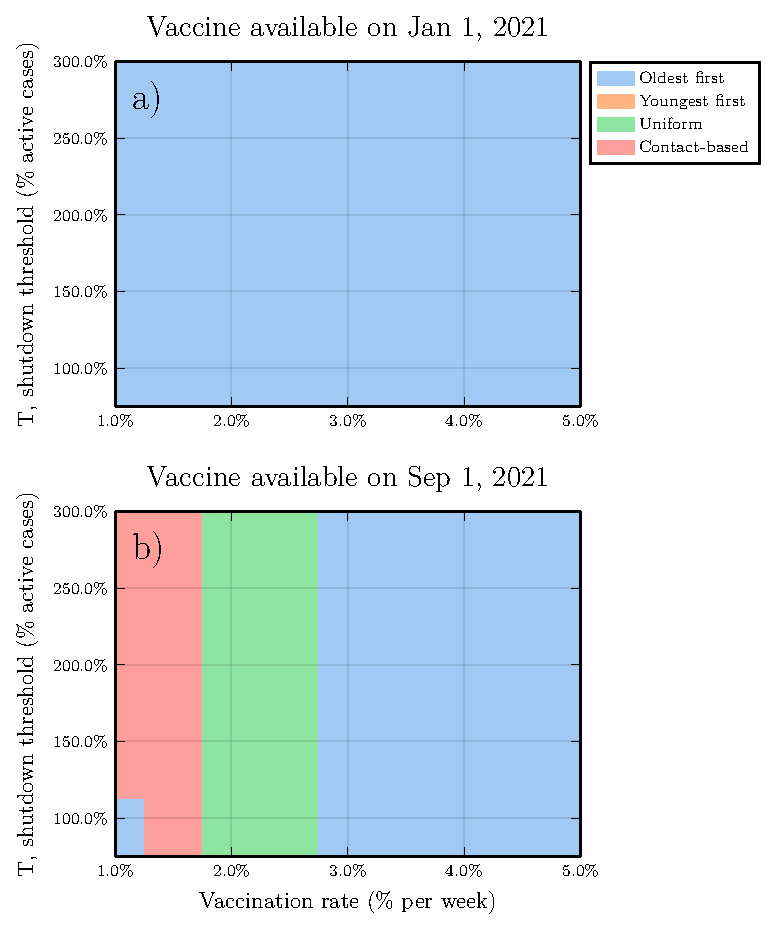
\includegraphics[width = 14 cm]{appendices/FigureS20.pdf}
    \caption[Sensitivity analysis for the scenario of $30 \%$ reduced ascertainment across all ages from December 2020 onward.]{\textbf{Sensitivity analysis for the scenario of $30 \%$ reduced ascertainment across all ages from December 2020 onward.} Subpanels are parameter planes for January and September availability showing the vaccination strategy that reduces COVID-19 mortality the most as a function of $T$ and $\psi_0$ (left) and the corresponding posterior parameter distributions for the refitted parameters (right).  Other parameter values as in Table S1.}
    \label{s20}
    \end{figure}
    
    \clearpage 
    
    
    \begin{figure}[H]
    \centering
    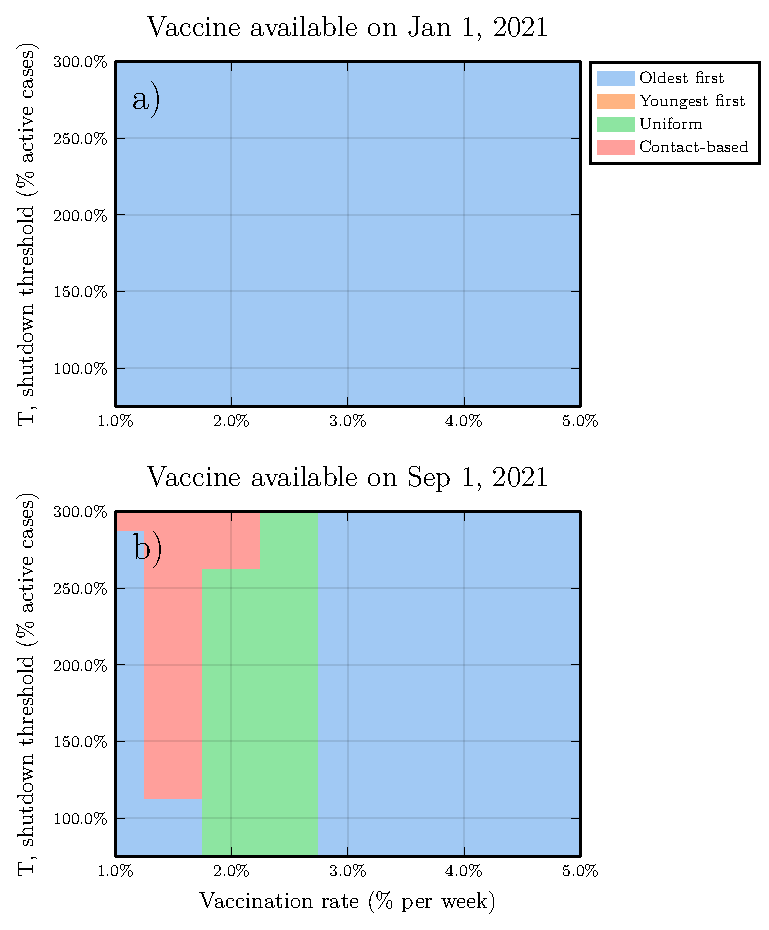
\includegraphics[width = 14 cm]{appendices/FigureS21.pdf}
    \caption[Sensitivity analysis for the scenario of four times the baseline social learning rate from December 2020 onward.]{\textbf{Sensitivity analysis for the scenario of four times the baseline social learning rate from December 2020 onward.} Subpanels are parameter planes for January and September availability showing the vaccination strategy that reduces COVID-19 mortality the most as a function of $T$ and $\psi_0$ (left) and the corresponding posterior parameter distributions for the refitted parameters (right).  Other parameter values as in Table S1.}
    \label{s21}
    \end{figure}
    
    \clearpage 
    
    \begin{figure}[H]
    \centering
    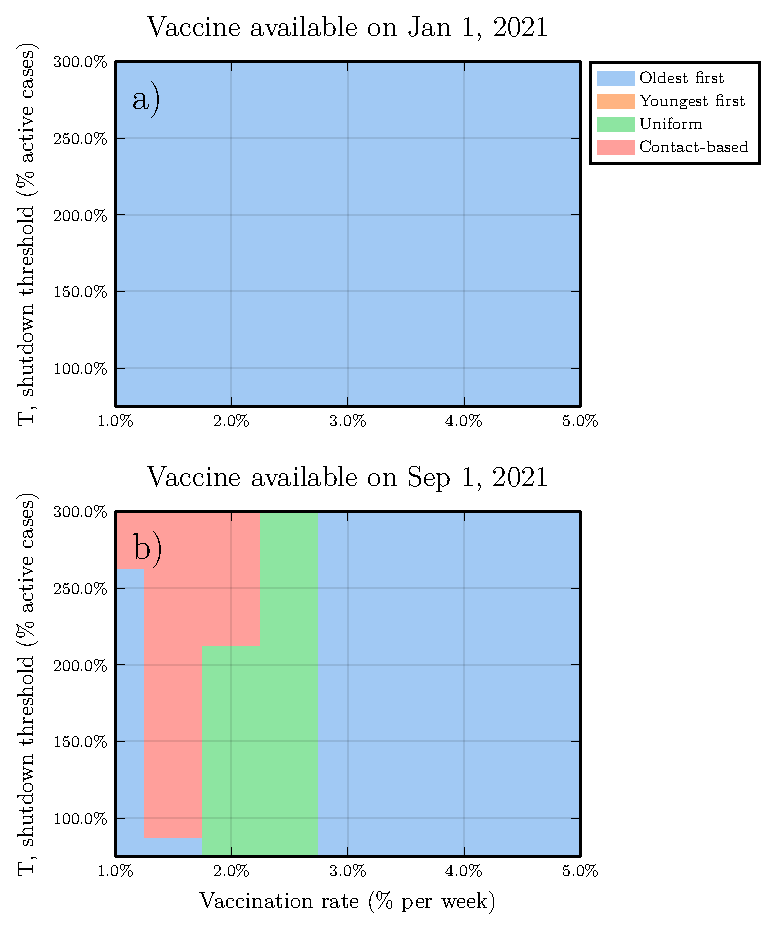
\includegraphics[width = 14 cm]{appendices/FigureS22.pdf}
    \caption[Sensitivity analysis for the scenario of one-fourth the baseline social learning rate from December 2020 onward.]{\textbf{Sensitivity analysis for the scenario of one-fourth the baseline social learning rate from December 2020 onward.} Subpanels are parameter planes for January and September availability showing the vaccination strategy that reduces COVID-19 mortality the most as a function of $T$ and $\psi_0$.  Other parameter values as in Table S1.}
    \label{s22}
    \end{figure}
    
    \clearpage 
    
    \begin{figure}[H]
    \centering
    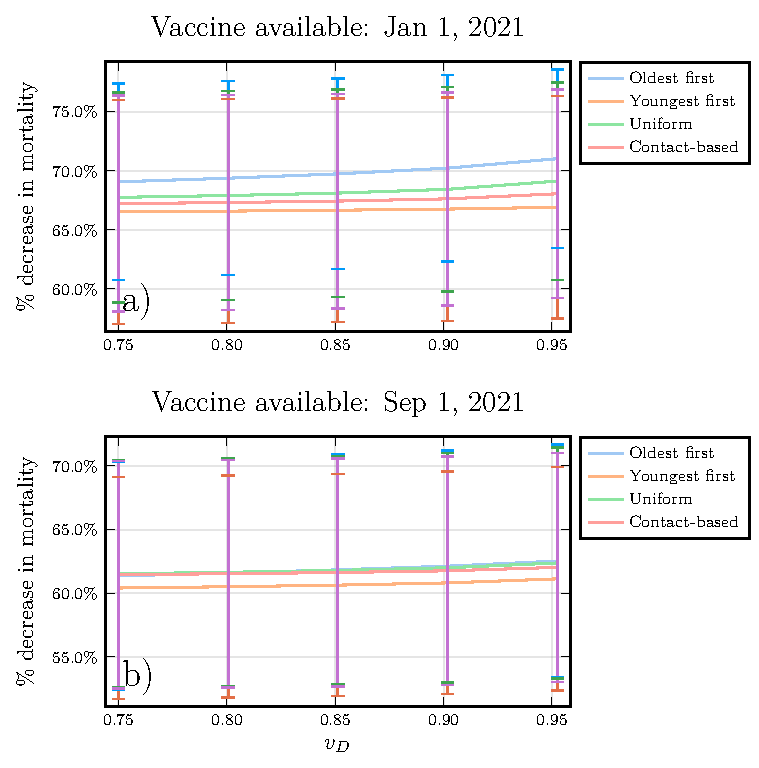
\includegraphics[width = 14 cm]{appendices/FigureS23.pdf}
    \caption[Sensitivity analysis for the scenario where efficacy against disease $v^D$ is not the same as efficacy against transmission $v^T$.]{\textbf{Sensitivity analysis for the scenario where efficacy against disease $v^D$ is not the same as efficacy against transmission $v^T$.} Subpanels show percentage reduction in mortality for the four stategies versus $v^D$ when $v^T=0.75$ but $v^D$ ranges from $0.75$ to $0.95$, for January and September availability.  Other parameter values as in Table S1.  Note that mortality in this plot is computed from March 15, 2020 to March 14, 2025.}
    \label{s23}
    \end{figure}
    
    \clearpage 
    
    
    \begin{figure}[H]
    \centering
    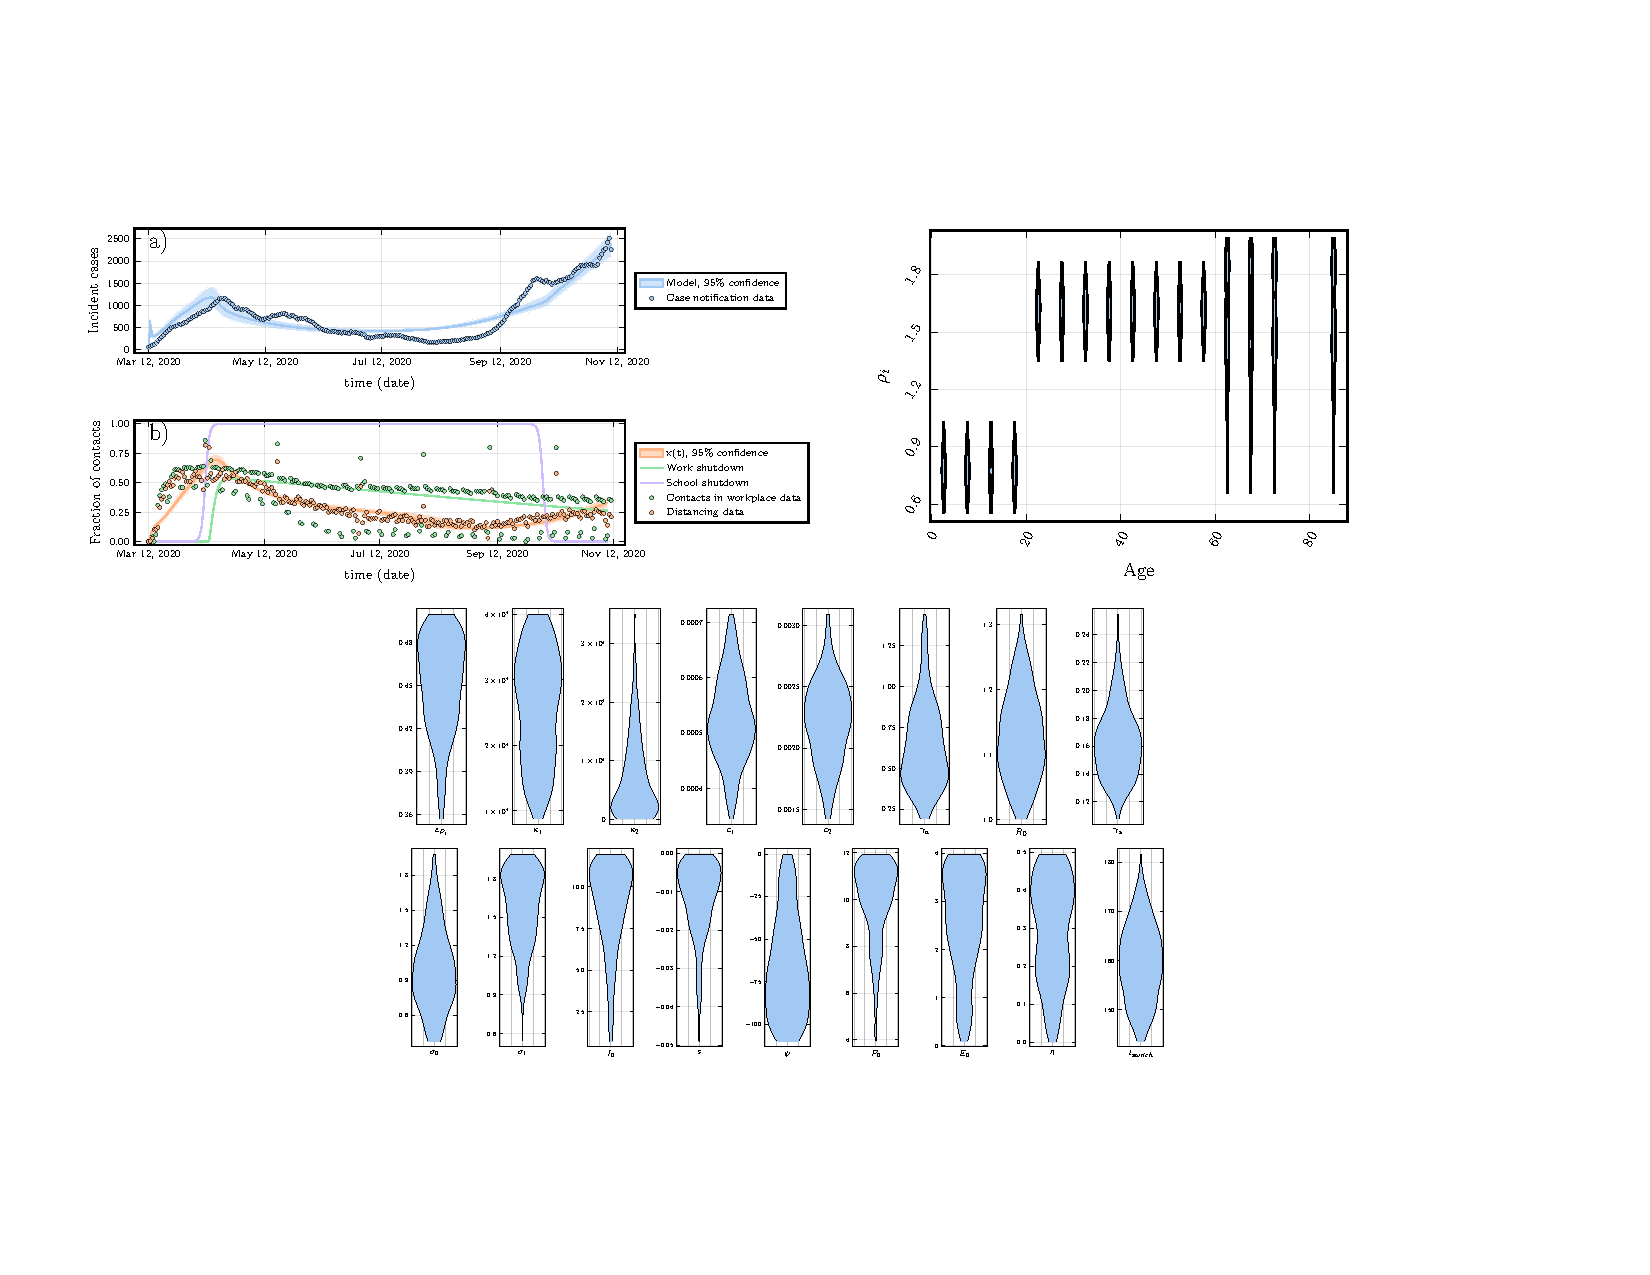
\includegraphics[width = 16 cm]{appendices/FigureS24.pdf}
    \caption[Posterior parameter distributions and model outputs for more stringent particle filtering criteria under Bayesian particle filtering algorithm.]{\textbf{Posterior parameter distributions and model outputs for more stringent particle filtering criteria under Bayesian particle filtering algorithm.} Top left panel shows (a) COVID-19 case incidence by date of report in Ontario, 7-day running average (circles) and ascertained case incidence from best fitting models (lines). (b) Percentage change from baseline in time spent at retail and recreation destinations (orange circles) and at workplaces (green circles) from Google mobility data, and proportion of the population x adhering to NPIs (orange line) and workplace shutdown curve (green line) from fitted model.  Top right panel shows posterior parameter distribution for age-specific susceptibility modifier, $\rho_i$ . Bottom panel shows other posterior parameter distributions. Other parameter values as in Appendix, pp. 1-11.}
    \label{s24}
    \end{figure}
    
    \begin{figure}[H]
    \centering
    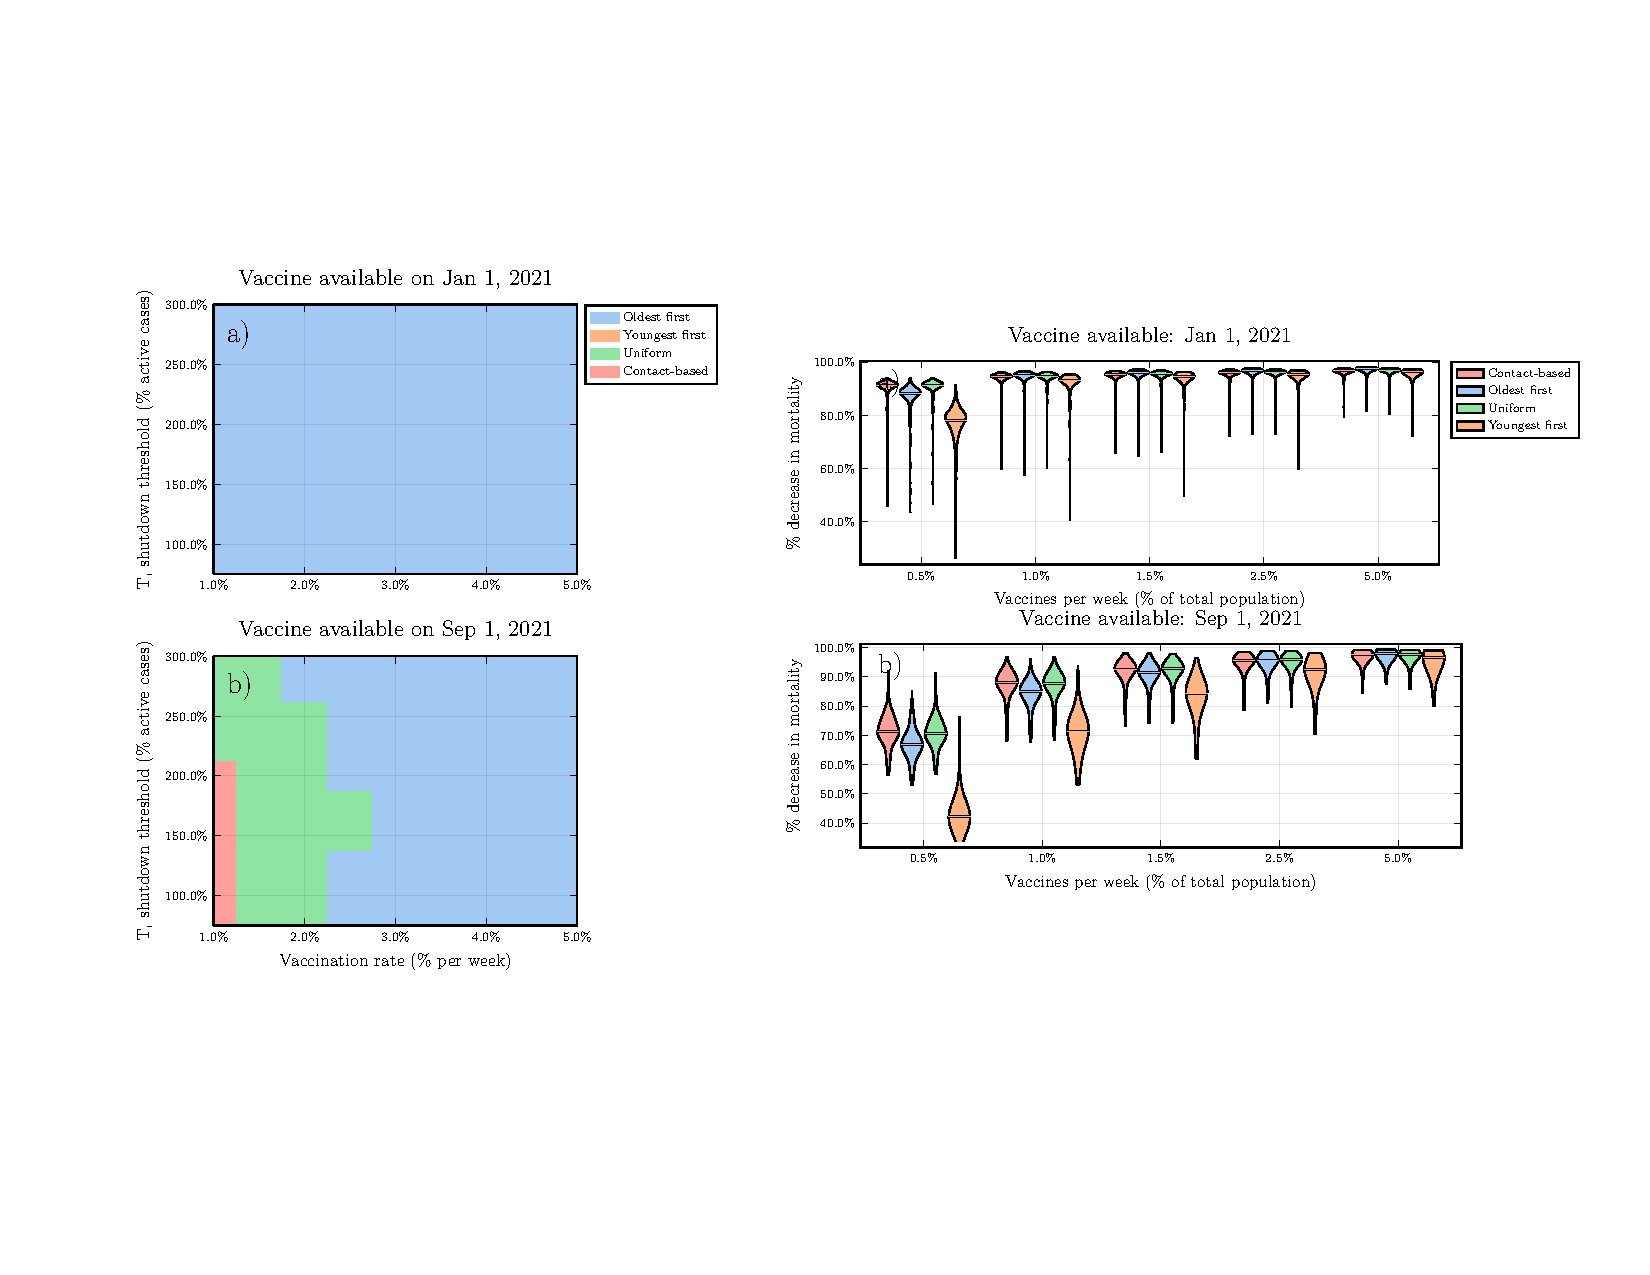
\includegraphics[width = 16 cm]{appendices/FigureS25.pdf}
    \caption[Sensitivity analysis for more stringent particle filtering criteria under Bayesian particle filtering algorithm.]{\textbf{Sensitivity analysis for more stringent particle filtering criteria under Bayesian particle filtering algorithm.} Subpanels are parameter planes for January and September availability showing the vaccination strategy that reduces COVID-19 mortality the most as a function of $T$ and $\psi_0$ (left) and violin plots showing percentage reduction in mortality (right).  Horizontal lines represent median values of posterior model projections. Shutdown threshold T=200 \% and other parameter values in Appendix, pp. 1-11. Percentage reductions are relative to no vaccination. Projected number of deaths in the absence of vaccination was 72,000 (95\% credible interval: 40,000 to 122,000) from January 1, 2021 to March 14, 2025 for (a) and 60,000 (95\% credible interval: 31,000 to 108,000) from September 1, 2021 to March 14, 2025 for (b).  Ontario Population size: 14.6 million.}
    \label{s25}
    \end{figure}
    
    \clearpage 
    
    \begin{figure}[H]
    \centering
    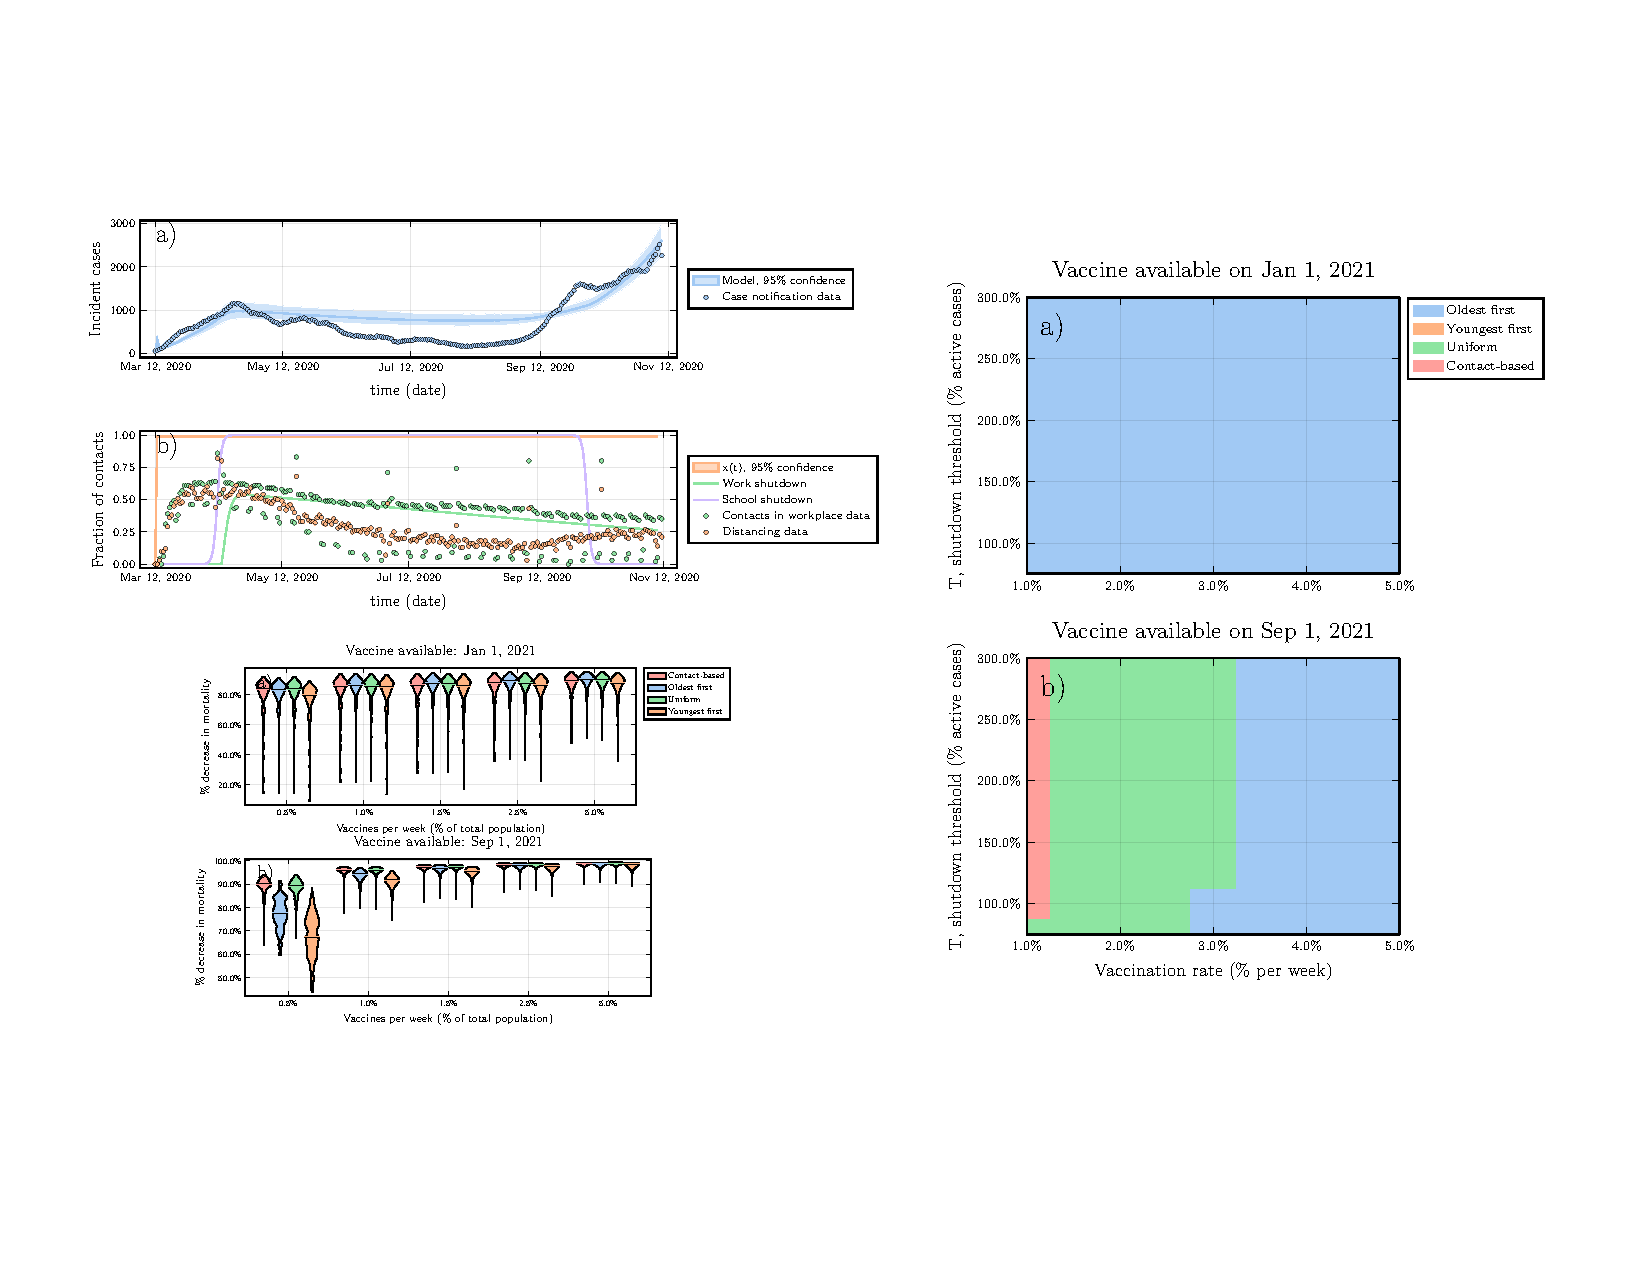
\includegraphics[width = 16 cm]{appendices/FigureS26.pdf}
    \caption[Model fit to data and baseline projections of mortality reductions under the four vaccine strategies, when behaviour is held constant over time.]{\textbf{Model fit to data and baseline projections of mortality reductions under the four vaccine strategies, when behaviour is held constant over time.} Top left: a) COVID-19 case incidence by date of report in Ontario, 7-day running average (circles) and ascertained case incidence from best fitting models (lines). (b) Percentage change from baseline in time spent at retail and recreation destinations (orange circles) and at workplaces (green circles) from Google mobility data, and proportion of the population x adhering to NPIs (orange line) and workplace shutdown curve (green line) from fitted model. Bottom left: Violin plots of the percent reduction in mortality under the four vaccine strategies, relative to no vaccination, as a function of the vaccination rate ψ0, for (a) January and (b) September 2021 availability. Horizontal lines represent median values of posterior model projections. Shutdown threshold T=200\%. Percentage reductions are relative to no vaccination. Projected number of deaths in the absence of vaccination was 72,000 (95\% credible interval: 40,000 to 122,000) from January 1, 2021 to March 14, 2025 for (a) and 60,000 (95\% credible interval: 31,000 to 108,000) from September 1, 2021 to March 14, 2025 for (b).  Ontario Population size: 14.6 million.  Right:  Each parameter combination on the plane is colour coded according to which of the four strategies prevented the most deaths, on average across all model realizations, for (a) January and (b) September 2021 availability. Other parameter values in Appendix, pp. 1-11.}
    \label{s26}
    \end{figure}
    
    \clearpage 
    
    \begin{figure}[H]
    \centering
    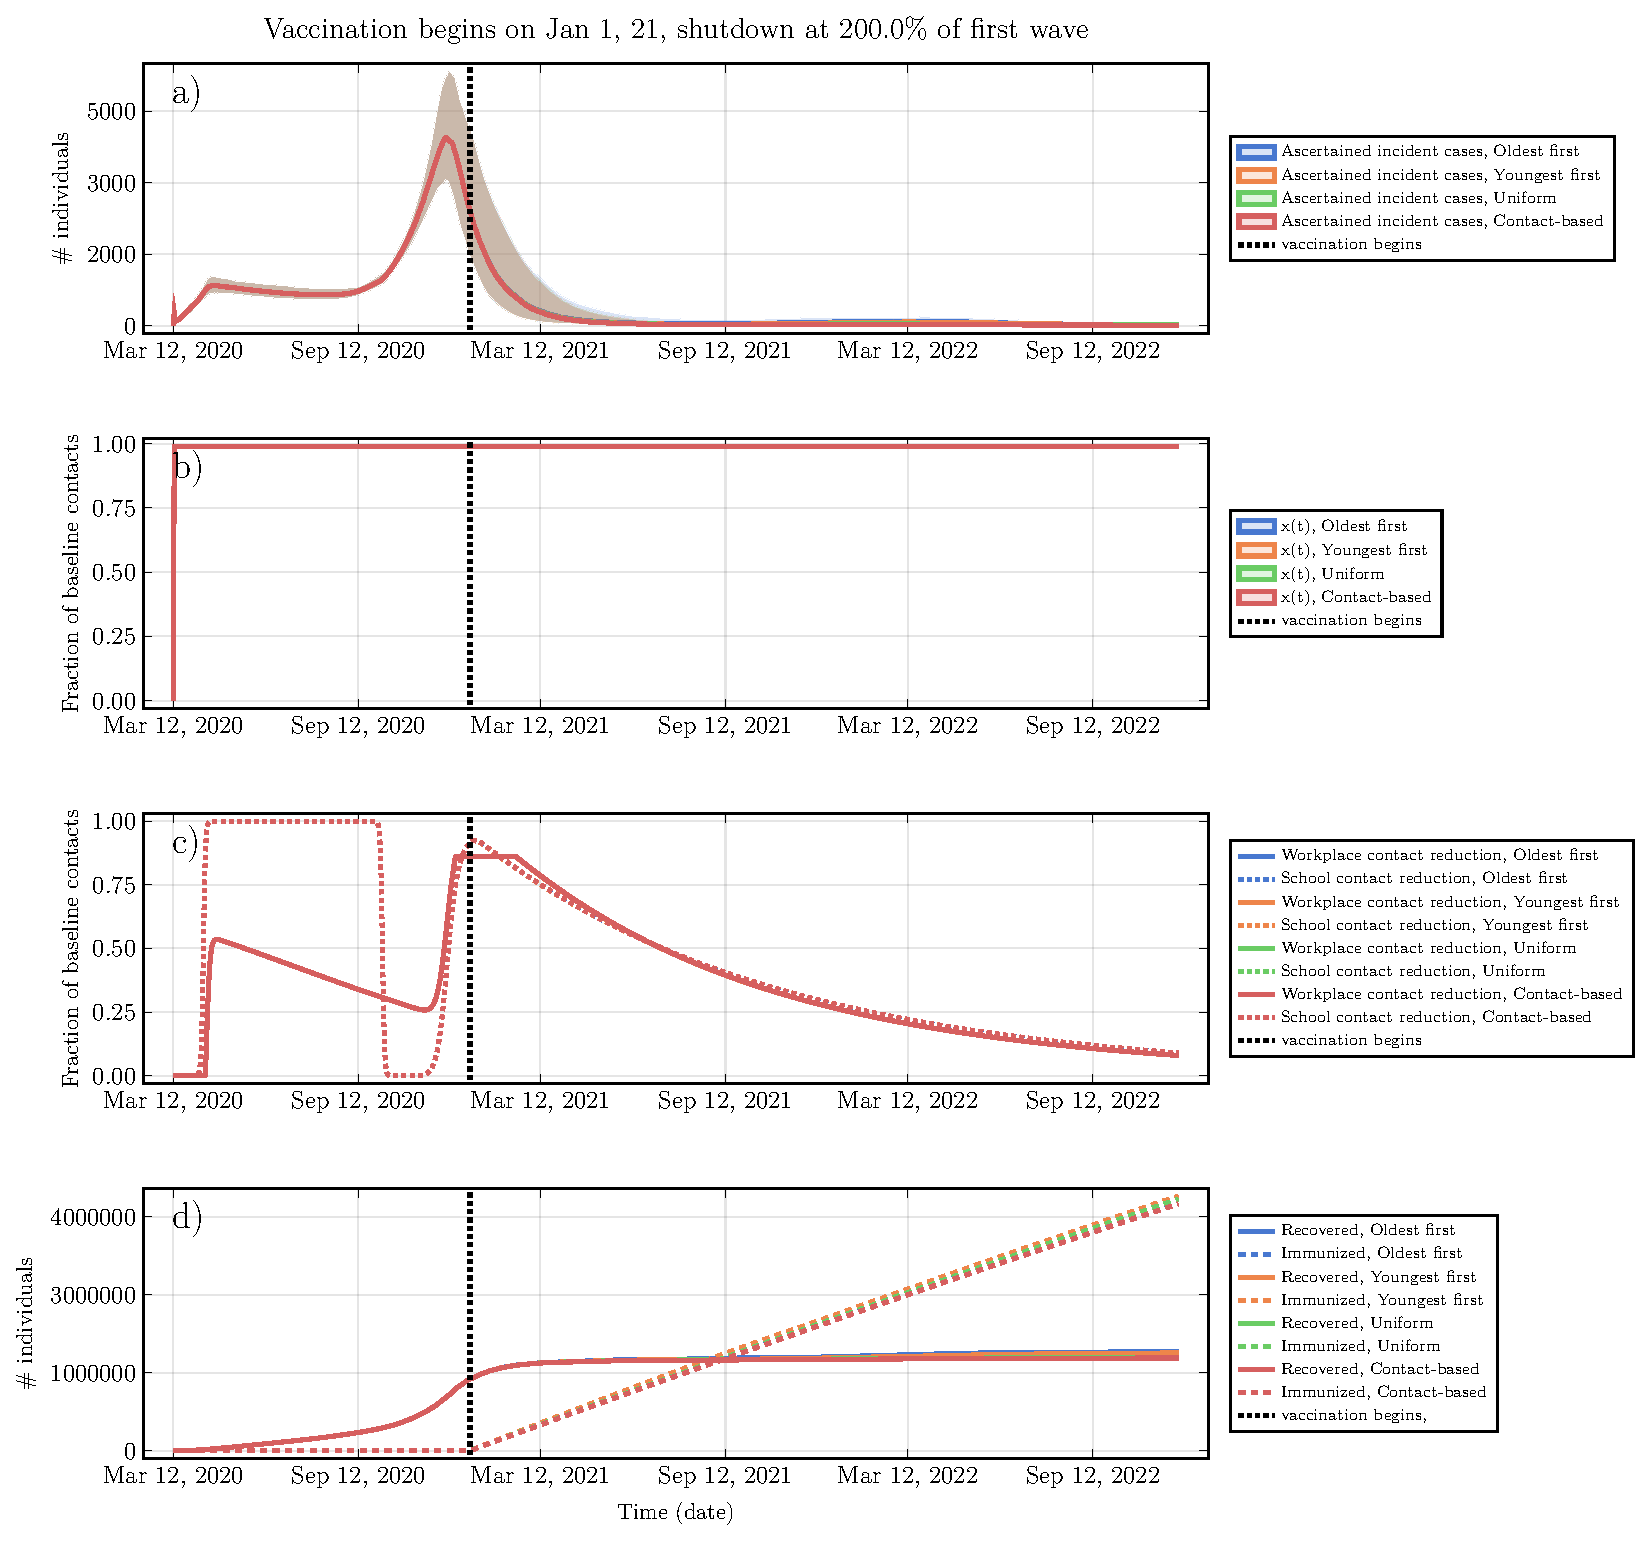
\includegraphics[width = 16 cm]{appendices/FigureS27.pdf}
    \caption[Epidemic dynamics and social dynamics for both NPI adherence and vaccinating behaviour, when behaviour is held constant over time.]{\textbf{Epidemic dynamics and social dynamics for both NPI adherence and vaccinating behaviour, when behaviour is held constant over time.} (a) Ascertained incident COVID-19 cases, (b) proportion $x$ of the population practicing NPIs, (c) Intensity of school and workplace closure, (d) percentage of population with natural or vaccine-derived immunity versus time. $T=200 \%$, $\psi_0=0.5 \%$ per week, vaccine available in January 2021. Other parameters are in Table \ref{tab:params}.}
    \label{s27}
    \end{figure}
    